%%
%% This is file `sample-sigplan.tex',
%% generated with the docstrip utility.
%%
%% The original source files were:
%%
%% samples.dtx  (with options: `all,proceedings,bibtex,sigplan')
%% 
%% IMPORTANT NOTICE:
%% 
%% For the copyright see the source file.
%% 
%% Any modified versions of this file must be renamed
%% with new filenames distinct from sample-sigplan.tex.
%% 
%% For distribution of the original source see the terms
%% for copying and modification in the file samples.dtx.
%% 
%% This generated file may be distributed as long as the
%% original source files, as listed above, are part of the
%% same distribution. (The sources need not necessarily be
%% in the same archive or directory.)
%%
%%
%% Commands for TeXCount
%TC:macro \cite [option:text,text]
%TC:macro \citep [option:text,text]
%TC:macro \citet [option:text,text]
%TC:envir table 0 1
%TC:envir table* 0 1
%TC:envir tabular [ignore] word
%TC:envir displaymath 0 word
%TC:envir math 0 word
%TC:envir comment 0 0
%%
%% The first command in your LaTeX source must be the \documentclass
%% command.
%%
%% For submission and review of your manuscript please change the
%% command to \documentclass[manuscript, screen, review]{acmart}.
%%
%% When submitting camera ready or to TAPS, please change the command
%% to \documentclass[sigconf]{acmart} or whichever template is required
%% for your publication.
%%
%%
\documentclass[sigconf]{acmart}


%%
%% \BibTeX command to typeset BibTeX logo in the docs
\AtBeginDocument{%
  \providecommand\BibTeX{{%
    Bib\TeX}}}
% \renewcommand\footnotetextcopyrightpermission[1]{}
%% Rights management information.  This information is sent to you
%% when you complete the rights form.  These commands have SAMPLE
%% values in them; it is your responsibility as an author to replace
%% the commands and values with those provided to you when you
%% complete the rights form.

\renewcommand\footnotetextcopyrightpermission[1]{}
\setcopyright{none}
% \setcopyright{acmcopyright}
\copyrightyear{2025}
\acmYear{2025}
\acmDOI{XXXXXXX.XXXXXXX}
%% These commands are for a PROCEEDINGS abstract or paper.
% \acmConference[RealSyn]{Preprint}
% \acmConference[\textit{RealSyn}]{October 28 - November 1,2024}{Preprint}
 \acmConference[\textit{RealSyn}]{ACM Conference}{Preprint}{}%
%%
%%  Uncomment \acmBooktitle if the title of the proceedings is different
%%  from ``Proceedings of ...''!
%%
%%\acmBooktitle{Woodstock '18: ACM Symposium on Neural Gaze Detection,
%%  June 03--05, 2018, Woodstock, NY}
% \acmISBN{978-1-4503-XXXX-X/YY/MM}


%%
%% Submission ID.
%% Use this when submitting an article to a sponsored event. You'll
%% receive a unique submission ID from the organizers
%% of the event, and this ID should be used as the parameter to this command.

%%
%% For managing citations, it is recommended to use bibliography
%% files in BibTeX format.
%%
%% You can then either use BibTeX with the ACM-Reference-Format style,
%% or BibLaTeX with the acmnumeric or acmauthoryear sytles, that include
%% support for advanced citation of software artefact from the
%% biblatex-software package, also separately available on CTAN.
%%
%% Look at the sample-*-biblatex.tex files for templates showcasing
%% the biblatex styles.
%%

%%
%% The majority of ACM publications use numbered citations and
%% references.  The command \citestyle{authoryear} switches to the
%% "author year" style.
%%
%% If you are preparing content for an event
%% sponsored by ACM SIGGRAPH, you must use the "author year" style of
%% citations and references.
%% Uncommenting
%% the next command will enable that style.
%%\citestyle{acmauthoryear}


%%
%% end of the preamble, start of the body of the document source.
\settopmatter{printacmref=false}
\usepackage{anyfontsize}
\usepackage{newfloat}
\usepackage{listings}
\usepackage{epsfig}
\usepackage{amsmath}
% \usepackage{amssymb}
\usepackage{bm}
\usepackage{algorithm}
\usepackage{algorithmic}
\usepackage{siunitx}
\usepackage{bbding}
\usepackage{pifont}
\usepackage{wasysym}
\usepackage{amsfonts}
\usepackage{mathtools}
\usepackage{makecell}
\usepackage{enumitem}
\usepackage{caption}
\usepackage{tcolorbox}
\usepackage{multirow}
\usepackage{colortbl}
\usepackage{subcaption}



\def\dsname{\textit{RealSyn}}
\definecolor{blue_ours}{HTML}{D8ECD1} 
\definecolor{green_ours}{rgb}{0.53, 0.83, 0.64}
\definecolor{dt}{gray}{0.7}
\definecolor{lightgray}{gray}{0.91}
\definecolor{cvprblue}{rgb}{0.21,0.49,0.74}

\newcommand{\tablestyle}[2]{\setlength{\tabcolsep}{#1}\renewcommand{\arraystretch}{#2}\centering\footnotesize}
\newcommand{\datatag}[1]{\rotatebox[origin=l]{90}{\small{#1}}}
\newcolumntype{x}[1]{>{\centering\arraybackslash}p{#1pt}}
\newcolumntype{y}[1]{>{\raggedright\arraybackslash}p{#1pt}}
\newcolumntype{z}[1]{>{\raggedleft\arraybackslash}p{#1pt}}
\newcommand{\app}{\raise.17ex\hbox{$\scriptstyle\sim$}}
\newcommand{\x}{{\times}}
\definecolor{baselinecolor}{gray}{.9}
\newcommand{\baseline}[1]{\cellcolor{baselinecolor}{#1}}
\newcolumntype{=}{>{\global\let\currentrowstyle\relax}}
\newcolumntype{^}{>{\currentrowstyle}}
\newcommand{\rowstyle}[1]{\gdef\currentrowstyle{#1}#1\ignorespaces}
\definecolor{dt}{gray}{0.2}  %

\definecolor{lightgray}{gray}{0.91}
\newcommand*{\belowrulesepcolor}[1]{% 
  \noalign{% 
    \kern-\belowrulesep 
    \begingroup 
      \color{#1}% 
      \hrule height\belowrulesep 
    \endgroup 
  }%
} 
\newcommand*{\aboverulesepcolor}[1]{% 
  \noalign{% 
    \begingroup 
      \color{#1}% 
      \hrule height\aboverulesep 
    \endgroup 
    \kern-\aboverulesep 
  }%
}
\begin{document}

\title{\includegraphics[width=0.5cm, height=0.7cm]{Figures/logo_crop.png} \textit{RealSyn}: An Effective and Scalable Multimodal Interleaved Document Transformation Paradigm}


\author{Tiancheng Gu$^\text{\ding{170}}$\textsuperscript{*}, Kaicheng Yang$^{\text{\ding{171}}}$\textsuperscript{*}, Chaoyi Zhang$^\text{\ding{170}}$, Yin Xie$^{\text{\ding{171}}}$, Xiang An$^{\text{\ding{171}}}$, \\ Ziyong Feng$^{\text{\ding{171}}}$, Dongnan Liu$^{\text{\ding{170}}}$, Weidong Cai$^{\text{\ding{170}}}$\textsuperscript{$\dagger$}, Jiankang Deng$^{\text{\ding{105}}}$\textsuperscript{$\dagger$}\\
$^{\text{\ding{170}}}$The University of Sydney $^{\text{\ding{171}}}$DeepGlint $^{\text{\ding{105}}}$Imperial College London \\
\texttt\tiny{tigu8498@uni.sydney.edu.au, kaichengyang@deepglint.com} \\
\textit{Homepage:\url{https://garygutc.github.io/RealSyn}}}
\thanks{\textsuperscript{*} Equal Contribution \\
\textsuperscript{$\dagger$} Corresponding Author}

\renewcommand{\shortauthors}{Tiancheng Gu, Kaicheng Yang et al.}


\begin{abstract}
\sloppy
After pre-training on extensive image-text pairs, Contrastive Language-Image Pre-training~(CLIP) demonstrates promising performance on a wide variety of benchmarks. However, a substantial volume of multimodal interleaved documents remains underutilized for contrastive vision-language representation learning. To fully leverage these unpaired documents, we initially establish a Real-World Data Extraction pipeline to extract high-quality images and texts. Then we design a hierarchical retrieval method to efficiently associate each image with multiple semantically relevant realistic texts. To further enhance fine-grained visual information, we propose an image semantic augmented generation module for synthetic text production. Furthermore, we employ a semantic balance sampling strategy to improve dataset diversity, enabling better learning of long-tail concepts. Based on these innovations, we construct \textit{RealSyn}, a dataset combining realistic and synthetic texts, available in three scales: 15M, 30M, and 100M. We compare our dataset with other widely used datasets of equivalent scale for CLIP training. Models pre-trained on \textit{RealSyn} consistently achieve state-of-the-art performance across various downstream tasks, including linear probe, zero-shot transfer, zero-shot robustness, and zero-shot retrieval. Furthermore, extensive experiments confirm that \textit{RealSyn} significantly enhances contrastive vision-language representation learning and demonstrates robust scalability. To facilitate future research, the \dsname\ dataset and pretrained model weights are released at \url{https://github.com/deepglint/RealSyn}.

\end{abstract}


%%
%% Keywords. The author(s) should pick words that accurately describe
%% the work being presented. Separate the keywords with commas.
\keywords{large-scale image-text dataset, vision-language representation learning, multimodal interleaved document}
%% A "teaser" image appears between the author and affiliation
%% information and the body of the document, and typically spans the
%% page.


% \received{20 February 2007}
% \received[revised]{12 March 2009}
% \received[accepted]{5 June 2009}

%%
%% This command processes the author and affiliation and title
%% information and builds the first part of the formatted document.
\maketitle

Stochastic systems have been used extensively in several areas including  verification~\cite{FKNP11}, learning theory~\cite{AJKS21}, epidemic processes~\cite{Lef81} to name a few. Several real-world systems however do not work with a centralised control. Therefore, modelling using stochastic systems with multiple agents makes for more faithful abstractions of such systems without a centralised control. Some examples of fields in which multi-agents stochastic modelling include cyber physical systems~\cite{SEC16}, distributed and probabilistic computer programs~\cite{dAHJ01}, probabilistic planning~\cite{TKI10}. In such cases, the problem of reasoning about multiple agents with several, often times orthogonal objectives, becomes important. % However, for situations that are modelled as graph games, Nash equilibria come with its own down-sides and therefore several notions of equilibria have emerged in turn-based games on graphs to circumvent the problems posed by the natural definitions of Nash equilibira, like subgame-perfect equilibira, Stackleberg-equilibria. 
For multi-agent systems modelled with stochasticity on the underlying arena, a fundamental question to ask is the existence or finding of an equilibrium.
The most popular equilibria in literature are Nash equilibria~\cite{Nas50}. However, those come with their own downsides. The computational complexity for studying Nash equilibria over multi-agent systems is prohibitively expensive, and even undecidable in the general case, where systems have $10$ or more players~\cite{UW11}. 
Further, even if Nash equilibria could be computed efficiently, they do not faithfully model the agents in real world settings
%as each agent might perceive risk differently. With randomness arising from both the strategies of other agents, as well as the underlying model of the system, this might mean that risk-averse or risk-loving agents might have an incentive to deviate since their perceived values of outcome is different from expected value of the game.
since they do not consider their tolerance or averseness to risk.

Let us consider a $1$-player game where a protagonist is proposed two options: (a) earning \$1; (b) playing a lottery in which, with probability $\frac{1}{40}$, she gets \$40, and with probability $\frac{39}{40}$, she does not earn anything.
Classically, rational strategies would be maximising the expected payoff. From this perspective, both options yield an expected payoff of \$1, making them equivalent.
This approach is particularly justified when the game represents a scenario that can be repeated many times: the law of large numbers ensures that, in the long run, the average payoff will converge to the expected payoff. However, when the game is played only once, the protagonist may prioritise immediate needs. If she urgently requires \$1, the guaranteed option (a) becomes preferable.

Conversely, if she is a risk-taker or finds herself in a situation where only the \$40 can make a significant difference, she may prefer the high-risk option (b).
Although this choice might appear irrational, it mirrors the behaviour of millions of people who participate everyday in games with a negative expected payoff, driven by the allure of a potentially life-changing win, and generating an annual turnover of USD 536 billions~\cite{GamblingNewspaper23} for the gambling industry.
That industry, on the other hand, operates on a large scale where expected payoff becomes the key metric. 
This contrast underscores the importance of alternative measures to expected payoff that account for each agent's risk tolerance.%, offering a more nuanced understanding of decision-making in uncertain scenarios.

%We thus have an example of a two-player interaction, with apparently zero-sum payoffs, but where both players express a preference for the same option, because the context gives them a different tolerance to risk: this paradox underscores the importance of alternative measures to expected payoff that account for an agent's risk tolerance, offering a more nuanced understanding of decision-making in uncertain scenarios.
% This contrast underscores the relevance of generalising the notion of Nash equilibria: in a multi-agent system, the agents may have diverging perception of which risks can be taken.
% It makes sense, then, to study \emph{risk-sensitive equilibria}, in which players do not necessarily maximise their expected payoff, but their perception of what their payoff will be according to different risk measures.\leon{I'm actually not satisfied with this, I will modify it and move it.}


% Classically, we consider that a rational strategy would consist in maximising the expected payoff: from that perspective, the two choices are equivalent.
% Such an approach is justified especially when the game models a situation that can be repeated a large number of times, in which case the law of large numbers guarantees that the average payoff converges to the expected payoff.
% But when the game models a situation that is played only once, the protagonist may consider that she really needs her euro, and that the possibility of earning 40\$ is too unlikely to be taken into account: she would then have a justifiable preference for the option (a).
% On the contrary, if she is more of a gambler, or if she finds herself in a desperate situation in which only earning those 40\$ could save her, she could go all out and express a strict preference for option (b)\footnote{Even though this case seems more irrational, it explain why millions of people play everyday games in which they know that their expected payoff is negative.
% On the other side, the companies with whom they interact repeat the experience often enough to consider expected payoff as the relevant measure --- generating a yearly turnover of 536 billions of US\$.}.
% Hence the relevance of alternatives to expected payoff, that take into account the tolerance of the agent to risk.

\subparagraph*{Risk Measures.}
A \emph{risk measure} captures the perception that a player has of what their payoff will be. In that sense, they generalise the notion of expected payoff.
Various risk measures exist in the literature, and have been used extensively in the field of economics and finance. 
Some of these risk measures include expected shortfall (ES), value at risk (VaR)~\cite{Aue18}, variance~\cite{Bra99}, entropic risk measure (ER)~\cite{FS02}. 

%However, since the introduction of the characteristic of risk measure called \emph{coherence}~\cite{ADJH99}, it was expected that a ``good'' a risk measure must be coherent. A risk measure is coherent if it is monotonic, homogeneous, translational-invariance, and sub-additive.
%This automatically weeds out several of the above risk measures listed above like  Value at Risk or variance as a risk measure. 
A lot of work has been done in considering these risk measures over MDPs which use variance (along with mean) as a risk-measure~\cite{FK89, PSB22,MT11}, ES~\cite{RRS15,KM18,Meg22} (also referred to as conditional value at risk (CVaR), average value at risk (AVaR), expected tail loss (ETL), and superquantile in literature) and ER~\cite{HM72,BR14,BCMP24}. % have also been studied. 
Studying the entropic risk measure in MDPs appears more practical compared to expected shortfall  or using variance-penalised risk-measures. This impracticability of ES and variance-penalised measure in particular is due to the intractable exponential memory~\cite{HK15} and time required to compute optimal strategies~\cite{PSB22}, even for the one agent system of Markov decision processes (MDPs). On the other hand, when the risk measure used is ER, players have optimal positional strategies in MDPs~\cite{How72}, which makes it a prime candidate for consideration in multi-agent settings.

\subparagraph*{Entropic Risk Measure.}
The entropic risk measure is computed by assigning to each agent a risk parameter, i.e., a value $\rho \in \Rb$.
%Based on this risk parameter $\rho$, this measure first computes the expectation of the exponential function of the random variable and then re-normalises this.  
The entropic risk measure of a random variable $X$ is then defined as
$\re_\rho[X] = -\frac{1}{\rho} \log_e \left( \Eb \left[ e^{-\rho X}\right] \right)$. 
%For computational reasons, instead of the Euler's constant $e$, we use different bases sometimes.
If the risk parameter $\rho$ is positive, then more weight will be given to the bad payoffs: the corresponding player can then be considered as risk-averse.
Conversely, players with a negative $\rho$ are more risk-loving.
When $\rho$ tends to $0$, the entropic risk measure converges to the classical expectation $\Eb[X]$.

The game depicted by Figure~\ref{fig:example_gamma} extends the lottery example we discussed earlier. 
Black vertices are stochastic, and the circle vertex is controlled by player $\Circle$.
A play can be seen as an infinite sequence of moves of a token along the edges of the graph, starting from $a$: from a stochastic vertex, it takes one of the outgoing edges with the probabilities indicated on those, and from a vertex controlled by the player, she chooses which edge it takes.
The payoff $40$, $0$, or $1$ is obtained when the terminal vertex $t_1$, $t_2$, or $t_3$ is reached, respectively.
If no terminal vertex is reached, then the payoff is $0$.
Taking the red edge corresponds to option (a): then, her risk entropy is always $1$, for every risk parameter $\rho$.
But if she chooses option (b), that is, if she takes the blue edge, her risk entropy is $\re_\rho[\mu_{\circ}] = -\frac{1}{\rho} \log \left( \Eb \left[ e^{-\rho \mu_{\circ}}\right] \right) = -\frac{1}{\rho} \log \left(  e^{-40\rho } + \frac{39}{40} \right)$.
Both cases are illustrated with red and blue curves in \cref{fig:example_plot}.
The curves cross at abscissa $\rho = 0$, where the entropic risk measure corresponds to the expectation. Note that other strategies are possible if \emph{randomisation} is allowed---the player could, for example, toss a coin and participate in the lottery if the outcome is heads. The perceived reward of randomising between outermost red and blue edges are illustrated in the intermediate cases with mixtures of red and blue in \cref{fig:example_plot}.

%For this example, we  replace Euler's constant $e$ with instead the constant $2$, which makes $\re_\rho[X] = -\frac{1}{\rho} \log_2 \left( \Eb \left[ 2^{-\rho X}\right] \right)$.

%Player $\Circle$ gets the payoff $11$ if she reaches the terminal vertex $t_1$, the payoff $1$ if she reaches $t_2$, the payoff $2$ if she reaches $t_3$, and the payoff $0$ if she reaches none of those terminal states (i.e., if she loops on the vertex $a$ forever).

%If the player's strategy is to choose the red edge, she gets payoff $1$ with probability $1$.
%Therefore, her risk measure is equal to $1$ for every risk parameter $\rho$.

%If her strategy is to choose the blue edge going to $c$, then she gets the payoff $11$ with probability $\frac{1}{10}$, and $1$ with probability $\frac{9}{10}$.
%Thus her risk entropy is
%$\re_\rho[\mu_{\circ}] = \frac{1}{\rho} \log_2\left(\frac{1}{3} 2^{-4\rho} + \frac{2}{3} 2^{-1\rho}\right)$.
 
\begin{figure}[h] 
			\centering
            \begin{subfigure}[t]{0.4\textwidth}
			\begin{tikzpicture}[->,>=latex,shorten >=1pt, initial text={}, scale=1, every node/.style={scale=1}]
				\node[initial left, stoch] (a) at (0, 0) {$a$};
				\node[state] (b) at (1.5, 0) {$b$};
                \node[stoch] (c) at (2.5, 1) {$c$};
                \node (t1) at (4, 2) {$t_1:~\stack{\circ}{40}$};
                \node (t2) at (4, 0) {$t_2:~\stack{\circ}{0}$};
                \node (t3) at (3, -1) {$t_3:~\stack{\circ}{1}$};
                \path (a) edge[loop above] node[above] {$\frac{1}{2}$} (a);
				\path (a) edge node[above] {$\frac{1}{2}$} (b);
                \path (b) edge[blue, thick] (c);
                \path (b) edge[red, thick] (t3);
				\path (c) edge node[above] {$\frac{1}{40}$} (t1);
				\path (c) edge node[below] {$\frac{39}{40}$} (t2);
			\end{tikzpicture}
			\caption{A stochastic MDP}
			\label{fig:example_gamma}
            \end{subfigure}
            \begin{subfigure}[t]{0.55\textwidth}
			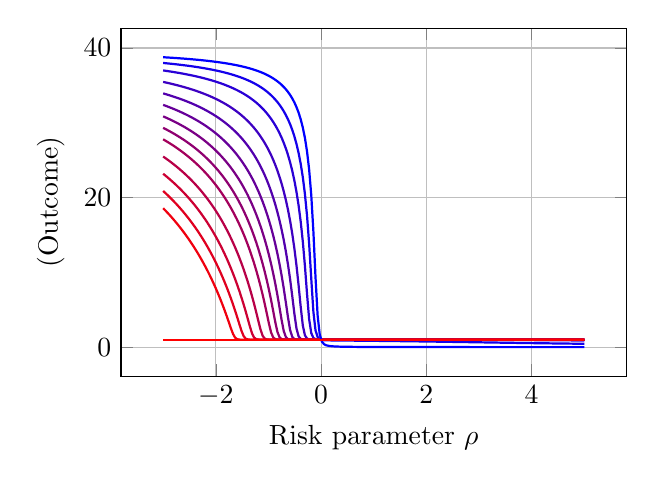
\begin{tikzpicture}
              \begin{axis}[
                xlabel={Risk parameter $\rho$},
                ylabel={$\re(\text{Outcome})$},
                domain=-3:5,
                samples=200,
                    width=8cm,
                   height=6cm,
                grid=major,
                ]
                \addplot [
                  red!8!blue,
                  thick
                ]
                {-1/x * log2((9/10)*e^(-1*x) + (1/400) * e^(-40*x) + (39/400))/log2(e)};
                \addplot [
                  red!16!blue,
                  thick
                ]
                {-1/x * log2((199/200)*e^(-1*x) + (1/8000) * e^(-40*x) + (39/8000))/log2(e)};
                \addplot [
                  red!24!blue,
                  thick
                ]
                {-1/x * log2((19999/20000)*e^(-1*x) + (1/800000) * e^(-40*x) + (39/800000))/log2(e)};
                \addplot [
                  red!32!blue,
                  thick
                ]
                {-1/x * log2((1999999/2000000)*e^(-1*x) + (1/80000000) * e^(-40*x) + (39/80000000))/log2(e)};
                \addplot [
                  red!40!blue,
                  thick
                ]
                {-1/x * log2((199999999/200000000)*e^(-1*x) + (1/8000000000) * e^(-40*x) + (39/8000000000))/log2(e)};
                \addplot [
                  red!48!blue,
                  thick
                ]
                {-1/x * log2((19999999999/20000000000)*e^(-1*x) + (1/800000000000) * e^(-40*x) + (39/800000000000))/log2(e)};
                \addplot [
                  red!56!blue,
                  thick
                ]
                {-1/x * log2((1999999999999/2000000000000)*e^(-1*x) + (1/80000000000000) * e^(-40*x) + (39/80000000000000))/log2(e)};
                \addplot [
                  red!64!blue,
                  thick
                ]
                {-1/x * log2((199999999999999/200000000000000)*e^(-1*x) + (1/8000000000000000) * e^(-40*x) + (39/8000000000000000))/log2(e)};
                \addplot [
                  red!72!blue,
                  thick
                ]
                {-1/x * log2((199999999999999999/200000000000000000)*e^(-1*x) + (1/8000000000000000000) * e^(-40*x) + (39/8000000000000000000))/log2(e)};
                \addplot [
                  red!80!blue,
                  thick
                ]
                {-1/x * log2((199999999999999999999/200000000000000000000)*e^(-1*x) + (1/8000000000000000000000) * e^(-40*x) + (39/8000000000000000000000))/log2(e)};
                \addplot [
                  red!88!blue,
                  thick
                ]
                {-1/x * log2((199999999999999999999999/200000000000000000000000)*e^(-1*x) + (1/8000000000000000000000000) * e^(-40*x) + (39/8000000000000000000000000))/log2(e)};
                \addplot [
                  red!94!blue,
                  thick
                ]
                {-1/x * log2((199999999999999999999999999/200000000000000000000000000)*e^(-1*x) + (1/8000000000000000000000000000) * e^(-40*x) + (39/8000000000000000000000000000))/log2(e)};
                \addplot [
                  blue,
                  thick
                ]
                {-1/x * log2((1/40) * e^(-40*x) + (39/40))/log2(e)};
                \addplot [
                  red,
                  thick
                ]
                {+1};
              \end{axis}
            \end{tikzpicture}
			\caption{Each curve represents the perceived reward of a player choosing only blue strategy, only red, or  randomising between both strategies. The percieved payoff for a player with risk parameter $\rho \in (-3,5)$ for these strategies are represented.}
			\label{fig:example_plot}
            \end{subfigure}
        \caption{Entropic risk measure}\label{fig:example_re}
\end{figure}
%\end{example}
Unfortunately, even for two player zero-sum stochastic games with total-reward objectives (payoff is the sum of the rewards seen along the way), computing optimal strategies can only be done in $\PSPACE$, when the base $e$ is replaced by an algebraic number; and if $e$ is the base of the exponent, then it is decidable only subject to Shanuel's conjecture~\cite{BCMP24}. % and inputs where the risk is computed using ER. 
Solving the two-player zero-sum case is a specific case of finding equilibria in two-agent systems where the payoffs of the two agents are exactly the negation of each others and so are the risk parameters of each of the agents.
Therefore, reasoning about multi-agent systems with ER also has potential to be computationally intractable.%\leon{I'm not sure I understand this sentence}


% \subparagraph*{Equilibria}
% Our example involves only one player.
% However, one might model it with a second player: the company that sells the lottery ticket, and therefore that made the choice of making the game possible.
% Of course, in the real world, companies only enable such games when its expected payoff is positive, that is, when the player's expected payoff is negative; which does not prevent millions of players to participate in such lotteries everyday, generating an annual turnover of USD 536 billion~\cite{h2_gambling_2023}.
% This can be explained by the fact that players are ready to take an important risk there, because they play a small number of times, and their likely loss remains acceptable, while their possible earning would be huge: in other words, players are efficiently modelled by a negative risk parameter.
% On the other hand, the company repeats the game a very large number of times, which is why, from its perspective, the expected payoff is the relevant metric.
% %This contrast underscores the importance of alternative measures to expected payoff that account for an agent's risk tolerance, offering a more nuanced understanding of decision-making in uncertain scenarios.
% This contrast underscores the relevance of generalising the notion of Nash equilibria: in a multi-agent system, the agents may have diverging perception of which risks can be taken.
% It makes sense, then, to study \emph{risk-sensitive equilibria}, in which players do not necessarily maximise their expected payoff, but their perception of what their payoff will be according to different risk measures.\leon{I'm actually not satisfied with this, I will modify it and move it.}



\subparagraph*{Extreme Risk Measure.} We introduce a new risk measure called extreme risk measure (XR) to identify tractable risk parameters. %\leon{Do we actually use that notation?} 
% If they have to choose between two options: (a) one which always gives him an outcome of 1, and the other option (b) that gives him a positive probability $p$ of 100, but  probability $(1-p)$ of -1, he would always chose option (a), 
%
%Let us say in a stochastic system, one agent is tasked with a safety-critical objective and wishes to avoid any positive probability of getting a payoff below some threshold, say $0$.
Consider an agent who wishes to maximise the lowest payoff received with positive probability.
In our example, 
by choosing option (a) her only payoff is $\$1$, whereas by choosing option (b), the payoffs that she receives with positive probability are $\$40$ and $\$0$. 
This agent would choose the option (a) since, then, the lowest reward she gets is $\$1$, instead of $\$0$. This would be her choice regardless of the probabilities or if the lottery amount in option (b) is increased.
%Even when the probabilities are changed for option (b) or if the lottery amount is increased, she would still prefer option (a).
Such agents can be considered ``extreme pessimists'' because
their perceived payoff can be thought of as the minimum among all the possible payoffs.
%We define the perceived reward of an extreme pessimist as the infimum of the payoffs that they get with positive probability. Therefore, extreme pessimists aim to maximise the smallest payoff that they receive with positive probability, and might be willing to deviate to achieve this objective.  
Similarly, one can define ``extreme optimists''  whose perceived reward is the best payoff that can be obtained with positive probability.
In the above scenario, an extreme optimist posed with the same options would choose option (b), no matter how small the probability is of receiving that payoff.

Extreme pessimists can be used to model safety-critical agents, where any positive probability of low reward or failure is unacceptable.
On the other hand, extreme optimists model naturally the opponents of such agents.
In a multiplayer setting, they can be an accurate modelling of agents like hackers in a system, who are happy with a small probability of success, or agents that have the possibility to restart their interactions with the same system, so that as long as there is a non-zero probability of achieving a high reward, they are guaranteed to receive that high reward. %\theju{If at all we discuss motivation here is the space.}





%\begin{example}
% Consider the same example game as in \cref{fig:example_gamma}. Here, the reward that the player perceives in the MDP can perceive on using the red strategy is exactly $2$ since that is the only payoff the player can get with a positive probability.
% However, if using the blue strategy, the perceived reward depends on if the player is an optimist or a pessimist. If the players is a pessimist, then the perceived reward is $4$, and if instead the player is an extreme pessimist, then the perceived reward is $1$.
%\end{example}
% \thejaswini{Introduce with examples some systems that need to be designed where some agent needs sure reward, and agents that some agents are happy with non-zero probability of reward}

%We capture this concept of extreme optimism and pessimism by introducing a new risk measure of pessimistic expectation and optimistic expectation.
\subparagraph*{Our results.}
We consider the problem of finding equilibria in a multiplayer stochastic game, that is, a game in which the payoffs that the players receive depend on the \emph{terminal vertex} that is reached, and in which an infinite play is associated to the zero payoff vector.

Our contributions are four fold. 
Firstly, we consider the problem of finding equilibria where entropic risk measure is used to determine the perceived reward of each player.  Each player has their own risk-sensitivity parameter, and we wish to find an equilibrium where no player has the incentive to deviate and increase their risk measure. We show that, when the rewards are all non-negative, such an equilibrium always exists.
We conjecture that this remains true when rewards can be negative.
Although some equilibria exist, not all equilibria are made the same, with some equilibria being more desirable than the others. One might want to find an equilibrium that maximises the overall social welfare, or want to minimise it for certain agents. A reasonably general setting is providing an interval for the risk measure for each agent and to check if there is an equilibrium satisfying these constraints. We call this problem \emph{constrained existence problem of risk-sensitive equilibria} (RSEs). 
We show (in \cref{sec:ERM}) that this problem is undecidable when the risk parameters of the players are rational values, with undecidability results extending from the constrained existence problem for Nash equilibria in the work of Ummels and Wojtczak~\cite{UW11}. However, we find restrictions on strategies to recover decidability. % for risk-sensitive equilibria in the cases where the risk parameters are finite.
If we restrict the memory requirements of each player, then for (small) finite memory strategies, we can solve the problem by encoding it using the existential theory of reals with exponentiation, giving us decidability subject to Shanuel's conjecture, and $\PSPACE$ algorithms when the base of the exponents are encoded as small algebraic instances, reminiscent of the two-player zero-sum case by Baier et al.~\cite{BCMP24}. 
%(\cref{proposition:Undecidable}).

Secondly, since the general problem is undecidable, and even in restricted cases, we obtain complexities that are $\PSPACE$ or higher, we pivot to searching for a more tractable risk measure that can be used to find equilibria in multi-agent systems. We define extreme risk measure (XR) as a novel risk measure to consider in multi-agent stochastic systems. We show (in \cref{sec:XR}) that our new definition is robust, since it exactly captures the well-studied entropic risk measure when the risk parameters tend to $\pm \infty$.
%This result (\cref{thm:RE=PEorOE}) in turn ensures that our risk measure is a robust definition since it is the limit of a well-studied risk measure. 
We further show the existence of 
such equilibria for games with non-negative rewards. Moreover, there exists a stationary strategy profile that can be algorithmically constructed in polynomial time. We conjecture, again, that this remains true when negative rewards are involved.
One further advantage of XR as a risk measure is that it is indifferent to the exact probabilities of the underlying stochastic model, since it only deals with events that occur with a positive probability and, therefore, can also be used in systems where the underlying probabilities are unknown. 

Thirdly, we show that the constrained existence problem of RSEs is decidable and also $\NP$-complete when the perceived payoff is calculated using XR, where each agent is either an extreme optimist or pessimist. The $\NP$ membership is nontrivial and follows several steps. First, we show that if there is a strategy that satisfies the constraints, then there is a finite abstraction of this strategy. Later, we show that this finite abstraction of the strategy has a polynomial representation. 
With this polynomial representation of the strategy, we show that verifying whether a given polynomially represented strategy is a risk-sensitive equilibrium that satisfies the constraints can also be done in polynomial time. 
Finally, we show that if all players are extreme optimists, this problem is $\PTIME$-complete.%, and provide a polynomial time algorithm for the constrained existence problem.
%\thejaswini{We add to this list by introducing a new risk measure that captures the above situation of extreme optimism and pessimism.}
%\thejaswini{We argue that our definition is robust, since this exactly captures the ERisk measure when the parameters are set to $-\infty$ and $+\infty$}
% \thejaswini{When the parameters are anywhere that are not $\pm\infty$, we show that computing Equilibria where ERisk is the outcome is undecidable. }
% \thejaswini{Argue that however, computational costs of precisely computing RSE for such values for stochastic games are undecidable}
% \thejaswini{This makes our definition the only decidable fragment for finding equilibria with entropic risk as a measure decidable}
\section{Related Work}
\label{sec:formatting}

\noindent{\bf Large-Scale Pre-training Dataset.} In recent years, several large-scale image-text datasets~\cite{MSCOCO, clark2017simple, goyal2017making, kakaobrain2022coyo700m, Densefusion1M} collected from the Internet have been released. The YFCC100M~\cite{YFCC100M} dataset provides a comprehensive overview of the evolution of photo and video documentation and sharing from the inception of Flickr in 2004 until early 2014. Due to download failures and non-English captions, DeCLIP~\cite{DECLIP} reprocesses a new version of the YFCC15M dataset. Additionally, the LAION400M~\cite{laion400M} dataset contains 400 million image-text pairs collected from Common Crawl and widely used in vision-language pre-training. Recent advancements have also introduced several large-scale interleaved image-text document datasets~\cite{omnicorpus, MMC4, Obelics}. The OBELICS~\cite{Obelics} dataset uses a comprehensive filtering strategy and includes 141 million web pages, 353 million associated images, and 115 billion text tokens extracted from Common Crawl. However, due to data format constraints and training inefficiencies, interleaved image-text documents are currently unsuitable for CLIP training.


\noindent{\bf Vision Language Pre-training.}
As a pioneering work in visual language pre-training, CLIP has attracted extensive attention due to its powerful zero-shot recognition and exceptional transfer learning performance~\cite{wang2024learn, tang2024amu, shao2024deil, martin2024transductive}. Inspired by CLIP, numerous visual-language pre-training works have been published in recent years~\cite{mu2022slip, DECLIP, ALIP}. SLIP~\cite{mu2022slip} enhances performance by combining self-supervised learning with CLIP pre-training. DeCLIP~\cite{DECLIP} increases pre-training efficiency by integrating multi-view supervision across modalities and nearest-neighbor supervision from similar pairs. To mitigate the influence of noisy data, ALIP~\cite{ALIP} introduces a gating mechanism that dynamically allocates weights to samples. Despite their advancements, these methods primarily depend on large-scale image-text pairs derived from the Internet. Recent studies~\cite{li2024scaling,wang2025scaling} demonstrate that the capabilities of CLIP enhance with the expansion of high-quality image-text datasets. Given the extensive use of internet-derived image-text data in existing datasets, there is a pressing need to develop a new data construction paradigm to further expand the scale of high-quality image-text data.


\noindent{\bf Synthetic Captions.} 
Recent works~\cite{ALIP, yu2024capsfusion, sharegpt4v} indicate that image-text pairs obtained from websites contain intrinsic noise, which directly impacts the effectiveness of vision-language pre-training. To enhance the quality of existing datasets, LaCLIP~\cite{laclip} uses the in-context learning capability of large language models to rewrite text descriptions associated with each image. CapsFusion~\cite{yu2024capsfusion} employs large language models to refine information from web-based image-text pairs and synthetic captions, improving the quality of multimodal pre-training data. 
Similarly, DreamLIP~\cite{DreamLIP} generates detailed descriptions for 30 million images using a pretrained large multimodal model. Nevertheless, these methods predominantly focus on synthetic data enhancement, neglecting the importance of real-world data. Furthermore, the diversity and distribution of synthetic captions generated by these methods are intrinsically constrained by the capabilities of the generative models employed.
\section{\textit{RealSyn} Dataset}

\subsection{Real-World Data Extraction}
To transform interleaved image-text documents for vision-language representation learning, we establish a Real-World Data Extraction pipeline~(Figure~\ref{fig: data_filtering}) to extract high-quality images and texts. This pipeline consists of three steps: Data Extraction, Image Filtration, and Sentence Filtration.

\noindent{\bf Data Extraction.} We employ 118M interleaved image-text documents from the OBELICS~\cite{Obelics} as the primary data source. All images are extracted and stored in a dedicated image database, while sentences are segmented using the Natural Language Toolkit (NLTK)~\cite{nltk} and stored in a separate sentence database. This process yields 336M images and 2.13B sentences from the interleaved documents.

\noindent{\bf Image Filtration.}
After extracting 336M images, we apply a two-stage filtering process to ensure data quality and reduce redundancy. First, we discard images that meet any of the following criteria: 1) the shorter dimension is fewer than 100 pixels, or 2) the aspect ratio exceeds 3 or is below 1/3. This step removes 51M low-quality images. Next, following CLIP-CID~\cite{CLIP_CID}, we use the EVA02-CLIP E/14-plus model~\cite{eva_clip} to extract image embeddings and apply the Union-Find algorithm~\cite{union_find} to eliminate perceptually and semantically redundant images. This step removes an additional 87M images, resulting in a refined dataset of 198M high-quality images.



\noindent{\bf Sentence Filtration.}
After extracting 2.13B sentences from interleaved image-text documents, we conduct rigorous filtering based on quality, semantics, and redundancy. Initially, we eliminate sentences based on the following criteria: 1) presence of emojis or URLs; 2) sentences containing fewer than 3 or more than 81 words; and 3) following CAT~\cite{CAT_rule}, we retain samples with at least C1 caption complexity and incorporating an action. This phase reduces the corpus size from 2.13B to 1.82B sentences. Then we apply semantic filtering to the remaining sentences, eliminating those with minimal information assessed through information entropy:
\begin{equation}
\label{equation:IE}
% \small
\theta(x) = -\sum_{i=1}^n p(x_{i}) \log p(x_{i}),
\end{equation}
where $n$ denotes the number of words in a sentence, $x_{i}$ represents the $i$-th words in the sentences $x$, and $p(x_{i})$ is the probability of the word $x_i$ in the entire corpus. Based on human cognition principles and empirical experience, we filter out sentences with a score below 0.3. To further refine the corpus by removing difficult or ambiguous sentences, we use GTP2-large~\cite{gpt2} to calculate the perplexity score $\mathcal{PPL}$ for each sentence:
\begin{equation}
\label{equation:perplexity}
% \small
\mathcal{PPL}(x) = \exp \left\{-\frac{1}{t} \sum_{i=1}^{t} \log p_{\theta}(x_i \mid x_{<i}) \right\},
\end{equation}
where $t$ represents the token number of the sentence, and $p_{\theta}(x_i \mid x_{<i})$ is the likelihood of the $i$-th token given the previous tokens. We engage three human experts to determine the minimum and maximum values of the perplexity interval for high-quality sentences by comparing sentences of varying perplexity levels. Sentences within the average minimum~(30) and maximum perplexity~(200) intervals are retained. The overall semantics filtering reduces the corpus to 1.16B sentences. In the final stage, similar to redundancy image filtering, we perform both perceptual and semantic deduplication of sentences. This process results in a refined corpus of 0.84B sentences that include extensive real-world knowledge.

\begin{figure}[t]
    \centering  \includegraphics[width=\linewidth]{Figures/framework.pdf}
    \vspace{-3mm}
    \caption{The architecture of our proposed framework, which constructs distinct image-text pairs from real-world data extracted from interleaved documents via retrieval and generation.}
    % \Description{}
    \label{fig: pipeline}
    \vspace{-3mm}
\end{figure}

\begin{table*}[t]
    \centering
    \caption{Linear probe on 20 downstream datasets. Pre-training ViT-B/32 on \dsname\ achieves 1.3\%-6.9\% average performance improvement.}
    \vspace{-2mm}
    \label{table:linear_probe}
    \resizebox{\linewidth}{!}{
    \begin{tabular}{cccccccccccccccccccccccc}
        \toprule
        \belowrulesepcolor{lightgray}
         \rowcolor{lightgray} Data Scale & Dataset & \rotatebox[origin=lb]{90}{\smash{Food101}} & \rotatebox[origin=lb]{90}{\smash{CIFAR10}} & \rotatebox[origin=lb]{90}{\smash{CIFAR100}} & \rotatebox[origin=lb]{90}{\smash{Birdsnap}} & \rotatebox[origin=lb]{90}{\smash{SUN397}} & \rotatebox[origin=lb]{90}{\smash{Cars}} & \rotatebox[origin=lb]{90}{\smash{Aircraft}} & \rotatebox[origin=lb]{90}{\smash{DTD}} & \rotatebox[origin=lb]{90}{\smash{Pets}} & \rotatebox[origin=lb]{90}{\smash{Caltech}} & \rotatebox[origin=lb]{90}{\smash{Flowers}} & \rotatebox[origin=lb]{90}{\smash{STL10}} & \rotatebox[origin=lb]{90}{\smash{EuroSAT}} & \rotatebox[origin=lb]{90}{\smash{RESISC45}} & \rotatebox[origin=lb]{90}{\smash{KITTI}} & \rotatebox[origin=lb]{90}{\smash{Country}} & \rotatebox[origin=lb]{90}{\smash{UCF101}} & \rotatebox[origin=lb]{90}{\smash{Memes}} & \rotatebox[origin=lb]{90}{\smash{SST2}} & \rotatebox[origin=lb]{90}{\smash{ImageNet}} & \rotatebox[origin=lb]{90}{\smash{\textbf{Average}}} \\
        \aboverulesepcolor{lightgray}
        \midrule
        \multirow{3}{*}{15M}
         & YFCC & 67.2 & 90.4 & 70.8 & \colorbox{blue_ours}{47.7} & 66.7& 23.8 & 29.7 & 62.4 & 65.7 & 80.1 & \colorbox{blue_ours}{90.0} & 94.7 & 94.9 & 79.4 & \colorbox{blue_ours}{75.4} & \colorbox{blue_ours}{18.4} & 70.8 & 48.6 & 56.2 & 56.7 & 64.5 \\
         & LAION &  71.0 & 93.3 & 78.1 & 41.0 & 66.3 & \colorbox{blue_ours}{76.9} & \colorbox{blue_ours}{43.0} & 71.2 & 74.5 & 87.6 & 88.2 & 93.6 & 95.3 & 82.9 & 72.2 & 13.5 & 75.4 & 55.7 & 57.3 & 59.3 & 69.8 \\
         & \dsname &  \colorbox{blue_ours}{77.1} & \colorbox{blue_ours}{94.5} & \colorbox{blue_ours}{78.7} & 43.4 & \colorbox{blue_ours}{71.4} & 64.7 & 42.7 & \colorbox{blue_ours}{71.3} & \colorbox{blue_ours}{79.9} & \colorbox{blue_ours}{90.0} & 88.2 & \colorbox{blue_ours}{96.4} & \colorbox{blue_ours}{96.2} & \colorbox{blue_ours}{87.2} & 72.4 & 16.7 & \colorbox{blue_ours}{79.9} & \colorbox{blue_ours}{55.7} & \colorbox{blue_ours}{57.7} & \colorbox{blue_ours}{64.0} & \colorbox{blue_ours}{71.4} \\
         \midrule
         \multirow{2}{*}{30M}
         & LAION& 76.1 & 94.5 & 80.0 & 47.4 & 70.3 & \colorbox{blue_ours}{82.3} & \colorbox{blue_ours}{45.9} & \colorbox{blue_ours}{74.7} & 80.3 & 89.8 & 89.5 & 95.6 & 95.5 & 84.5 & 72.6 & 15.2 & 76.6 & \colorbox{blue_ours}{56.2}& \colorbox{blue_ours}{60.0} & 64.3 & 72.6 \\
         % & Merged & 78.6 & 95.2 & 81.5 & 47.9 & 73.2 & 76.6 & 43.4 & 74.5 & 80.8 & 90.6 & 89.3 & 96.8 & 95.7 & 87.5 & 72.6 & 17.4 & 80.5 & \colorbox{blue_ours}{57.0} & 59.4 & 66.4 & 73.2 \\
         & \dsname & \colorbox{blue_ours}{81.2} & \colorbox{blue_ours}{95.4} & \colorbox{blue_ours}{81.8} & \colorbox{blue_ours}{48.4} & \colorbox{blue_ours}{74.5} & 73.4 & 45.2 & 74.2& \colorbox{blue_ours}{84.1} & \colorbox{blue_ours}{91.3} & \colorbox{blue_ours}{90.6} & \colorbox{blue_ours}{97.2} & \colorbox{blue_ours}{96.5} & \colorbox{blue_ours}{89.2} & \colorbox{blue_ours}{74.5} & \colorbox{blue_ours}{19.0} & \colorbox{blue_ours}{82.6} & 55.0 & 56.2 & \colorbox{blue_ours}{68.5} & \colorbox{blue_ours}{73.9} \\
         \midrule
         \multirow{2}{*}{100M}
         & LAION& 80.2 & 95.7 & 82.5 & 51.3 & 73.4 & \colorbox{blue_ours}{85.3} & 46.1 & 75.6 & 83.2 & 91.1 & \colorbox{blue_ours}{92.0} & 96.9 & 95.2 & 85.9 & 68.4 & 17.4 & 80.0 & 57.3& \colorbox{blue_ours}{61.4} & 68.3 & 74.4 \\
         & \dsname & \colorbox{blue_ours}{84.2} & \colorbox{blue_ours}{96.3} & \colorbox{blue_ours}{83.5} & \colorbox{blue_ours}{54.0} & \colorbox{blue_ours}{76.2} & 77.4 & \colorbox{blue_ours}{47.6} & \colorbox{blue_ours}{75.6} & \colorbox{blue_ours}{86.3} & \colorbox{blue_ours}{92.1} & 91.7 & \colorbox{blue_ours}{97.7} & \colorbox{blue_ours}{96.8} & \colorbox{blue_ours}{90.6} & \colorbox{blue_ours}{73.1} & \colorbox{blue_ours}{21.1} & \colorbox{blue_ours}{83.7} & \colorbox{blue_ours}{57.3} & 58.9 & \colorbox{blue_ours}{71.6} & \colorbox{blue_ours}{75.8} \\
        \bottomrule
    \end{tabular}
    }    
\vspace{-2mm}
\end{table*}
\begin{table*}[t!]
    \centering
    \caption{Zero-shot transfer on 20 downstream datasets. Pre-training ViT-B/32 on \dsname\ achieves 2.3\%-14.3\% average performance improvement.}
    \vspace{-2mm}
    \label{table:zeroshot_classfication}
    \resizebox{\linewidth}{!}{
    \begin{tabular}{cccccccccccccccccccccccc}
        \toprule
        \belowrulesepcolor{lightgray}
        \rowcolor{lightgray} Data Scale &  Dataset & \rotatebox[origin=lb]{90}{\smash{Food101}} & \rotatebox[origin=lb]{90}{\smash{CIFAR10}} & \rotatebox[origin=lb]{90}{\smash{CIFAR100}} & \rotatebox[origin=lb]{90}{\smash{Birdsnap}} & \rotatebox[origin=lb]{90}{\smash{SUN397}} & \rotatebox[origin=lb]{90}{\smash{Cars}} & \rotatebox[origin=lb]{90}{\smash{Aircraft}} & \rotatebox[origin=lb]{90}{\smash{DTD}} & \rotatebox[origin=lb]{90}{\smash{Pets}} & \rotatebox[origin=lb]{90}{\smash{Caltech}} & \rotatebox[origin=lb]{90}{\smash{Flowers}} & \rotatebox[origin=lb]{90}{\smash{STL10}} & \rotatebox[origin=lb]{90}{\smash{EuroSAT}} & \rotatebox[origin=lb]{90}{\smash{RESISC45}} & \rotatebox[origin=lb]{90}{\smash{KITTI}} & \rotatebox[origin=lb]{90}{\smash{Country}} & \rotatebox[origin=lb]{90}{\smash{UCF101}} & \rotatebox[origin=lb]{90}{\smash{Memes}} & \rotatebox[origin=lb]{90}{\smash{SST2}} & \rotatebox[origin=lb]{90}{\smash{ImageNet}} & \rotatebox[origin=lb]{90}{\smash{\textbf{Average}}} \\
        \aboverulesepcolor{lightgray}
        \midrule
        \multirow{3}{*}{15M} 
        & YFCC & 36.3 & 74.0 & 40.3 & \colorbox{blue_ours}{19.4} & 41.8 & 2.1 & 2.3 & 12.0 & 19.8 & 59.8 & \colorbox{blue_ours}{48.9} & 87.7 & 21.2 & 20.3 & 23.8 & 5.1 & 27.8 & 47.4 & 50.1 & 32.3 & 33.6 \\
         & LAION & 49.1 & 85.7 & 56.9 & 11.5 & 45.1 & \colorbox{blue_ours}{49.9} & 3.8 & 25.7 & 54.6 & 78.1 & 30.5 & 89.5 & 36.7 & 36.1 & 21.7 & 5.6 & 38.2 & 48.8 & 49.9 & 37.1 & 42.7 \\
         & \dsname & \colorbox{blue_ours}{60.0} & \colorbox{blue_ours}{85.7} & \colorbox{blue_ours}{58.3} & 10.5 & \colorbox{blue_ours}{56.4} & 27.6 & \colorbox{blue_ours}{5.5} & \colorbox{blue_ours}{33.2} & \colorbox{blue_ours}{61.7} & \colorbox{blue_ours}{80.2} & 31.2 & \colorbox{blue_ours}{92.4} & \colorbox{blue_ours}{56.5} & \colorbox{blue_ours}{56.2} & \colorbox{blue_ours}{34.0} & \colorbox{blue_ours}{8.9} & \colorbox{blue_ours}{52.6} & \colorbox{blue_ours}{53.3} & \colorbox{blue_ours}{51.3} & \colorbox{blue_ours}{43.3} & \colorbox{blue_ours}{47.9} \\
         \midrule
         \multirow{2}{*}{30M} 
         & LAION & 58.9 & 85.9 & 63.1 & \colorbox{blue_ours}{17.4} & 54.8 & \colorbox{blue_ours}{61.0} & 4.3 & 36.4 & 65.5& 82.0 & 41.3 & 91.3 & 40.3 & 43.7 & 24.3 & 7.2 & 47.4 & 51.5 & 50.1 & 44.9 & 48.6 \\
         & \dsname & \colorbox{blue_ours}{67.5} & \colorbox{blue_ours}{89.0} & \colorbox{blue_ours}{65.2} & 15.0 & \colorbox{blue_ours}{60.6} & 39.2 & \colorbox{blue_ours}{7.9} & \colorbox{blue_ours}{37.8} & \colorbox{blue_ours}{70.5} & \colorbox{blue_ours}{84.0} & \colorbox{blue_ours}{42.2} & \colorbox{blue_ours}{93.8} & \colorbox{blue_ours}{59.9} & \colorbox{blue_ours}{61.9} & \colorbox{blue_ours}{27.7} & \colorbox{blue_ours}{10.6} & \colorbox{blue_ours}{56.7} & \colorbox{blue_ours}{52.5} & \colorbox{blue_ours}{50.1} & \colorbox{blue_ours}{50.9} & \colorbox{blue_ours}{52.1} \\
         \midrule
         \multirow{2}{*}{100M} 
         & LAION & 68.9 & \colorbox{blue_ours}{90.5} & 68.6 & \colorbox{blue_ours}{23.6} & 60.6 & \colorbox{blue_ours}{68.3} & 7.8 & 41.2 & 74.7 & 87.1 & 47.7 & 94.4 & 45.6 & 53.4 & 23.6 & 10.4 & 54.5 & 51.9 & 53.3 & 52.8 & 53.9 \\
         & \dsname & \colorbox{blue_ours}{73.5} & 89.5 & \colorbox{blue_ours}{68.8} & 20.1 & \colorbox{blue_ours}{65.0} & 48.5 & \colorbox{blue_ours}{10.2} & \colorbox{blue_ours}{46.1} & \colorbox{blue_ours}{76.7} & \colorbox{blue_ours}{87.6} & \colorbox{blue_ours}{48.8} & \colorbox{blue_ours}{94.4} & \colorbox{blue_ours}{69.0} & \colorbox{blue_ours}{65.5} & \colorbox{blue_ours}{24.6} & \colorbox{blue_ours}{12.1} & \colorbox{blue_ours}{60.5} & \colorbox{blue_ours}{52.4} & \colorbox{blue_ours}{54.1} & \colorbox{blue_ours}{56.2} & \colorbox{blue_ours}{56.2} \\
        \bottomrule
    \end{tabular}
    }
\vspace{-2mm}
\end{table*} 

\subsection{\bf Retrieval and Generation Framework} 
After extracting high-quality images and sentences from documents, we propose an efficient and scalable framework to retrieve multiple semantically relevant texts for each image and leverage large language models to integrate retrieved realistic text with fine-grained visual information and generate synthetic text. As shown in Figure~\ref{fig: pipeline}, the architecture of our framework primarily consists of three components: Text Semantic Clustering, Hierarchical Retrieval, and Image Semantic Augmented Generation.



\noindent{\bf Text Semantic Clustering.} To efficiently retrieve multiple semantically relevant texts for each image, we initially encode all sentences using the EVA02-CLIP E/14-plus~\cite{eva_clip} model. Inspired by Unicom~\cite{unicom}, we utilize the standard $K$-Means algorithm~\cite{kmeans} offline cluster all sentences into a specified number of clusters. To minimize intra-cluster and inter-cluster conflicts, we initially establish the optimal number of cluster centroids through small-scale experiments. Subsequently, we divide the 0.84 billion texts into two million clusters, utilizing efficient feature quantization techniques~\cite{johnson2019billion}.

\noindent{\bf Hierarchical Retrieval.} Given the prohibitive computational cost of direct semantic text retrieval across 0.84B sentences (requiring over 10,000 GPU-hours on 8×A100), we propose a hierarchical retrieval framework to enhance efficiency. Given an image, we perform inter-cluster retrieval to identify the most relevant cluster center for the image. Subsequently, we conduct intra-cluster retrieval within the identified cluster to obtain multiple real-world sentences semantically matched to the image. This approach achieves scalable retrieval of 198M images and 0.84B sentences within 40 GPU-hours on an 8×A100.


\noindent{\bf Image Semantic Augmented Generation.} Although the retrieved realistic texts achieve satisfactory performance, they exhibit limitations in capturing fine-grained visual semantics. To address this issue, we introduce the Image Semantic Augmented Generation module. This module initially employs the OFA~\cite{OFA} model to generate a concise caption for each image. We then integrate the open-set image tagging model RAM++~\cite{RAM_plus_plus}, which extracts object detection tags. Considering that RAM++ supports only 4,000 tags, we expand this set to 8,000 by incorporating an additional 4,000 tags derived from real-world sentences. Following CapsFusion~\cite{yu2024capsfusion}, we utilize ChatGPT4 Turbo to merge the retrieved realistic texts with concise captions and image tags to construct a 100K instruction dataset (the prompt we used is presented in the supplementary material). Subsequently, we conduct instruction tuning of the LLaMA3-8B model~\cite{llama3} using the LLaMA Factory~\cite{llamafactory} and deploy the vLLM~\cite{vLLM} for large-scale inference. Ultimately, we convert data from 118M multimodal interleaved documents into 198M image-text pairs, where each image is associated with multiple retrieved realistic texts and synthetic texts.

\begin{table*}[t!]
\centering
\caption{Zero-shot image-text retrieval performance on Flickr30k and MSCOCO. Pre-training CLIP-B/32 on \dsname\ dataset achieves a significant improvement on all metrics.}
% \vspace{-2mm}
\label{tab:retrieval}
\resizebox{0.95\linewidth}{!}{
    \centering
    \begin{tabular}{cccccccccccccc}
    \toprule
    \belowrulesepcolor{lightgray}
     \rowcolor{lightgray}  & &\multicolumn{6}{c}{Text Retrieval} & \multicolumn{6}{c}{Image Retrieval} \\
     \rowcolor{lightgray}  & &\multicolumn{3}{c}{Flickr30k} & \multicolumn{3}{c}{MSCOCO} & \multicolumn{3}{c}{Flickr30k} & \multicolumn{3}{c}{MSCOCO} \\
     \rowcolor{lightgray} Data Scale & Dataset& R@1 & R@5 & R@10 & R@1 & R@5 & R@10 & R@1 & R@5 & R@10 & R@1 & R@5 & R@10 \\
    \aboverulesepcolor{lightgray} %  
    \midrule \multirow{3}{*}{15M} 
    & YFCC & 37.1 & 64.8 & 75.9 & 21.3 & 45.1 & 57.0 & 23.5 & 47.3 & 58.3 & 13.2 & 32.0 & 43.1 \\
    & LAION & 49.1 & 76.8 & 84.5 & 28.4 & 53.0 & 64.9 & 33.3 & 60.5 & 70.9 & 17.4 & 38.3 & 49.7 \\
    & \dsname & \colorbox{blue_ours}{72.9} & \colorbox{blue_ours}{91.1} & \colorbox{blue_ours}{95.1} & \colorbox{blue_ours}{43.8} & \colorbox{blue_ours}{69.5} & \colorbox{blue_ours}{79.6} & \colorbox{blue_ours}{49.5} & \colorbox{blue_ours}{76.3} & \colorbox{blue_ours}{84.6} & \colorbox{blue_ours}{25.8} & \colorbox{blue_ours}{50.6} & \colorbox{blue_ours}{62.5} \\
    \midrule \multirow{2}{*}{30M} 
    & LAION & 59.6 & 83.5 & 89.8 & 35.9 & 62.4 & 73.2 & 42.4 & 70.1 & 79.4 & 22.1 & 45.5 & 57.6 \\
    & \dsname & \colorbox{blue_ours}{76.0} & \colorbox{blue_ours}{93.3} & \colorbox{blue_ours}{96.9} & \colorbox{blue_ours}{48.2} & \colorbox{blue_ours}{74.6} & \colorbox{blue_ours}{83.0} & \colorbox{blue_ours}{54.0} & \colorbox{blue_ours}{80.0} & \colorbox{blue_ours}{87.6} & \colorbox{blue_ours}{29.5} & \colorbox{blue_ours}{55.2} & \colorbox{blue_ours}{66.9} \\
    \midrule \multirow{2}{*}{100M} 
    & LAION & 67.5 & 87.9 & 93.0 & 43.3 & 68.0 & 78.1 & 50.4 & 77.2 & 85.5 & 27.1 & 52.1 & 63.8\\
    & \dsname & \colorbox{blue_ours}{81.6} & \colorbox{blue_ours}{96.1} & \colorbox{blue_ours}{97.3} & \colorbox{blue_ours}{52.3} & \colorbox{blue_ours}{76.7} & \colorbox{blue_ours}{85.0} & \colorbox{blue_ours}{58.8} & \colorbox{blue_ours}{84.1} & \colorbox{blue_ours}{90.5} & \colorbox{blue_ours}{32.5} & \colorbox{blue_ours}{58.9} & \colorbox{blue_ours}{70.2} \\
    \bottomrule
    \end{tabular}
    }
\vspace{-1mm}
\end{table*}


\begin{table}[t!]
\centering
\caption{Zero-shot robustness comparison on different IN-1K val set variants. Pre-training CLIP-B/32 on \dsname\ demonstrates superior robustness across all datasets.}
% \vspace{-2mm}
\label{tab:robustness}
\resizebox{\linewidth}{!}{
    \begin{tabular}{cccccccc}
        \toprule
        \belowrulesepcolor{lightgray}
        \rowcolor{lightgray} Data Scale  & Dataset& IN-V2 & IN-A & IN-R  & ObjectNet & IN-Sketch & \textbf{Average}\\
        \aboverulesepcolor{lightgray} % 
        \midrule \multirow{3}{*}{15M} 
        & YFCC & 27.3 & 12.3 & 20.8 & 25.3 & 6.3 & 18.4  \\
        & LAION & 30.7 & 6.0 & 46.5 & 28.7 & 24.3 & 27.2  \\
        & \dsname & \colorbox{blue_ours}{37.1} & \colorbox{blue_ours}{12.5} & \colorbox{blue_ours}{47.7} & \colorbox{blue_ours}{35.0} & \colorbox{blue_ours}{25.4} & \colorbox{blue_ours}{31.5}  \\
        \midrule \multirow{2}{*}{30M} 
        & LAION & 37.5 & 8.9 & 54.4 & 35.5 & 31.8 & 33.6  \\
        & \dsname & \colorbox{blue_ours}{42.9} & \colorbox{blue_ours}{16.1} & \colorbox{blue_ours}{56.6} & \colorbox{blue_ours}{41.5} & \colorbox{blue_ours}{31.9} & \colorbox{blue_ours}{37.8}  \\
        \midrule \multirow{2}{*}{100M} 
        & LAION & 44.6 & 12.2 & 62.5 & 42.2 & 37.9 & 39.9  \\
        & \dsname & \colorbox{blue_ours}{47.6} & \colorbox{blue_ours}{19.7} & \colorbox{blue_ours}{62.5} & \colorbox{blue_ours}{45.8} & \colorbox{blue_ours}{37.9} & \colorbox{blue_ours}{42.7}  \\
	\bottomrule
    \end{tabular}
    }
\vspace{-6mm}
\end{table}

\subsection{Semantic Balance Sampling}
To further improve the quality and diversity of our dataset, we implement semantic balancing sampling across the 198M image-text pairs. Specifically, we use EVA02-CLIP E/14-plus~\cite{eva_clip} to encode and calculate the cosine similarity between images and synthetic texts. To reduce the impact of OCR-related or mismatched pairs during pre-training, we filter out 29.7M pairs with cosine similarities scores either above 0.61 or below 0.51, as determined through human verification. Inspired by MetaCLIP~\cite{xu2023metaclip}, we introduce an easy but efficient cluster-based semantic balance sampling strategy. We cluster the image embeddings from the remaining 168.3M pairs into 1M centers. To enhance the semantic diversity of our dataset, we randomly select 20, 35, and 180 samples from clusters exceeding these thresholds, while retaining all samples from smaller clusters.  This approach culminates in the construction of the \dsname15M, \dsname30M, and \dsname100M datasets.






\section{Experiments and Results}




\subsection{Implementation Details}
We initially collect 118M interleaved image-text documents from the OBELICS~\cite{Obelics} as our primary data source. We use OFA$_{base}$~\cite{OFA} and RAM++$_{large}$~\cite{RAM_plus_plus} to generate brief captions and semantic tags. To validate the dataset performance, we pre-train standard CLIP supervised by the text randomly selected from the three retrieved realistic texts and one synthetic text, inspired by the LaCLIP~\cite{laclip}. During pre-training, we adopt AdamW~\cite{AdamW} as the optimizer, with a learning rate of 1e-3 and a weight decay of 0.2. The parameters $\beta1$ and $\beta2$ are set to 0.9 and 0.98, respectively. The input image size is 224×224, and the input text sequence length is 77. The temperature parameter $\tau$ is initialized to 0.07. We train 32 epochs with 4096 batch sizes on 8 $\times$ A100 (80G) GPUs. Please refer to the supplementary material for more details.

To validate the effectiveness of the \dsname\ dataset, we compare \dsname\ with the previous datasets across various models and data scales. We compare \dsname15M with the YFCC15M filtered by DeCLIP~\cite{DECLIP}. Following ALIP~\cite{ALIP}, we also compare with LAION15M, LAION30M, and LAION100M~(subset randomly selected from LAION400M).


\begin{figure*}[t!]
    \centering
    \includegraphics[width=\linewidth]{Figures/topic_distribution_V2.pdf}
    \vspace{-6mm}
    \caption{A T-SNE~\cite{tsne} projection of LDA~\cite{LDA} topic cluster from a randomly selected 1M samples from \dsname. \dsname\ encompasses a broad range of everyday topics, e.g., animal, food, airplane, etc. We also display representative central images for each identified topic.}
    \vspace{-2mm}
    \label{fig: dataset_topic_distribution}
\end{figure*}

\subsection{Main Results}
\label{main_result}
\noindent{\bf Linear Probe.} In Table~\ref{table:linear_probe}, we report the linear probe performance of the ViT-B/32 model across 20 downstream datasets. When pretrained at the 15M scale, \dsname15M exceeds YFCC15M on 16 of 20 datasets, achieving an average performance increase of 6.9\%. Additionally, \dsname15M outperforms LAION15M on 18 of 20 datasets, with an average improvement of 1.6\%. With dataset scaling to 30M and 100M, \dsname\ achieves average performance improvements of 1.3\% and 1.4\% over LAION, respectively. These findings underscore the superior CLIP training efficiency of the \dsname\ dataset compared to the widely-used YFCC and LAION datasets across multiple scales.

\noindent{\bf Zero-shot Transfer.} We evaluate the zero-shot transfer performance of the ViT-B/32 model across 20 classification benchmarks using the same prompt templates as SLIP~\cite{mu2022slip}. As indicated in Table~\ref{table:zeroshot_classfication}, \dsname15M surpasses YFCC15M on 18 of 20 datasets, achieving an average performance improvement of 14.3\%. In comparison to LAION15M, \dsname15M excels on 18 of 20 datasets with an average improvement of 5.2\%. Upon expanding the dataset sizes to 30M and 100M, \dsname\ achieves average performance improvements of 3.5\% and 2.3\% compared to LAION, highlighting its efficiency and scalability.

It is important to note that \dsname\ demonstrates a significant decrease in performance on certain datasets, such as Cars and Flowers. This reduction is primarily attributed to the unique data distribution of \dsname, characterized by a scarcity of data for specific concepts, which hampers the model’s ability to effectively learn these concepts. For example, as shown in Figure~\ref{fig: dataset_topic_distribution}, samples related to cars and flowers represent only 0.9\% and 0.4\% of the dataset, respectively.


\noindent{\bf Zero-shot Image-Text Retrieval.} In Table~\ref{tab:retrieval}, we present the zero-shot image-text retrieval performance of the ViT-B/32 model pre-trained on different scales of datasets. \dsname\ achieves superior results across all evaluation metrics. Specifically, \dsname15M improves Recall@1 by 35.8\%\&26\% on Flickr30K~\cite{flickr30k} and by 22.5\%\&12.6\% on MSCOCO~\cite{mscoco_retrieval}. \dsname30M improves Recall@1 by 16.4\%\&11.6\% on Flickr30K~\cite{flickr30k} and by 12.3\%\&7.4\% on MSCOCO~\cite{mscoco_retrieval}. \dsname100M
improves Recall@1 by on 14.6\%\&8.4\% Flickr30K~\cite{flickr30k} and by 9\%\&5.4\% on MSCOCO~\cite{mscoco_retrieval}. This significant enhancement in cross-modal retrieval performance indicates that the \dsname\ dataset effectively improves contrastive vision-language representation learning by incorporating both realistic and synthetic texts, resulting in robust representations and enhanced cross-modal alignment.



\noindent{\bf Zero-shot Robustness.} To further validate the robustness of the \dsname\ dataset, we present the zero-shot robustness~\cite{CLIP} performance across various IN-1K~\cite{ImageNet} val set variants in Table~\ref{tab:robustness}. The results indicate that \dsname\ significantly enhances the robustness of vision-language pre-training models. Specifically, \dsname15M shows a performance increase of 13.1\% and 4.3\% compared to YFCC15M and LAION15M, respectively. When scaled to 30M and 100M, \dsname\ achieves additional improvements of 4.2\% and 2.8\% over LAION. This substantial enhancement in performance is primarily attributable to the utilization of retrieved realistic texts, which surpass the constraints of generative models, and the superior conceptual diversity relative to YFCC and LAION, thus significantly boosting model robustness.



\begin{figure}[!t]
\centering
    \begin{subfigure}{0.22\textwidth}
    \includegraphics[width=1.0\textwidth]{Figures/image_captioning/coco2017_name.png}
    \end{subfigure}
    \begin{subfigure}{0.22\textwidth}
    \includegraphics[width=1.0\textwidth]{Figures/image_captioning/flickr30K_name.png}
    \end{subfigure}
\vspace{-3mm}
\caption{Image captioning comparisons on COCO2017 and Flickr30k. B4, MT., RL. and Cd. represent the metric of BLEU~\cite{BLEU}, METEOR~\cite{METEOR}, ROUGE-L~\cite{METEOR}, and Cider~\cite{cider}.}
% \Description{}
\vspace{-3mm}
\label{image_captioning}
\end{figure}

\noindent{\bf Image Captioning via MLLM.} In Figure~\ref{image_captioning}, we present the image captioning performance of the LLaVA-1.5~\cite{llava1.5} trained using different datasets (LAION v.s. \dsname). Initially, we first map visual features into the textual domain using the initial 558k dataset from LLaVA-1.5. We then develop an image captioning dataset from both LAION and \dsname\ for instruction tuning. Specifically, we select 1M samples randomly from each dataset and train over two epochs. As depicted in Figure~\ref{image_captioning}, \dsname\ significantly outperforms LAION in all evaluation metrics on both the COCO2017~\cite{mscoco_retrieval} and Flickr30k~\cite{flickr30k} benchmarks. This notable performance enhancement confirms the higher quality and better image-text alignment of the \dsname\ dataset.


\begin{figure}[t!]
\centering
\begin{subfigure}{\linewidth}
{
\includegraphics[height=0.48\textwidth]{Figures/data_distribution/data_consine_similarity_analysis.png}}
{
\includegraphics[height=0.48\textwidth]{Figures/data_distribution/data_token_len.png}}
\caption{Richness assessment comparison}
\label{similarity_token}
\end{subfigure}

\begin{subfigure}{\linewidth}
\centering
\includegraphics[width=\linewidth]{Figures/data_richness/diversity_analysis.png}
\vspace{-7mm}
\caption{Diversity assessment comparison}
\label{fig:diversity}
\end{subfigure}
\vspace{-5mm}
\caption{The richness assessment and diversity assessment on different datasets. \dsname-R1: the most relevant retrieved realistic text. \dsname-S1: the semantic augmented synthetic text based on \dsname-R1.}
\vspace{-3mm}
\end{figure}

\section{Analysis}

\begin{figure}[t!]
\centering
\includegraphics[width=\linewidth]{Figures/data_scaling_law.png}
\vspace{-5mm}
\caption{Data Scaling Analysis. We pretrain ViT-B/32 on \dsname\ in different data scales. \textcolor{red}{$\times$} represents the results predicted using our data scaling law.}
% \Description{}
\label{fig:data_scaling_analysis}
\vspace{-2mm}
\end{figure}

\subsection{Statistics Analysis} 
\noindent{\bf Topic-based Assessment.} Following MMC4~\cite{MMC4}, we ran LDA~\cite{LDA} on random sampling 1M image-realistic text pairs with 30 topics. Figure~\ref{fig: dataset_topic_distribution} presents the proportions and examples for six topics: animal, food, airplane, flower, automotive, and landmark. Notably, the dataset contains minimal samples related to ``flower'' and ``automotive'' topics, representing merely 0.4\% and 0.9\% of the total, respectively. This paucity of examples hinders the model's ability to sufficiently learn these concepts, thereby compromising its performance in the linear probe and zero-shot transfer evaluations on the Flowers and Cars datasets.


\noindent{\bf Richness Assessment.} Figure~\ref{similarity_token} presents image-text similarity and text token distribution of 15M samples from YFCC15, LAION, \dsname-R1 (the most relevant retrieved realistic text), and \dsname-S1 (the semantic augmented synthetic text based on \dsname-R1). Compared to datasets sourced from the Internet, \dsname\ demonstrates robust similarity metrics even after the removal of OCR data. This effectively explains the significant performance enhancement observed in the CLIP model trained on \dsname\ for image-text retrieval tasks.  Moreover, both the retrieved realistic texts and synthetic texts contain a larger quantity of words, which can provide a richer textual context that enhances vision-language representation learning.


\noindent{\bf Diversity Assessment.} The \dsname\ is constructed based on real-world interleaved image-text documents, which encompasses a wide array of diverse information. Following previous work~\cite{lai2024revisit}, we randomly select 0.2M samples to calculate the number of unique entities in the caption to assess the data diversity of different datasets. As depicted in Figure~\ref{fig:diversity}, both the retrieved realistic texts and image semantic augmented synthetic texts exhibit a higher number of distinct entities. Such diversity enriches the dataset, facilitating the model's acquisition of comprehensive knowledge and enhancing both performance and robustness.



\noindent{\bf Data Scaling Analysis.} We present the data scaling law~\cite{scaling_law} derived from our \dsname\ dataset, justifying its scalability over samples.
Specifically, we conduct a series of visual-language pre-trainings with proposed datasets ranging from 12M to 60M, and fit each performance metric to the inverse of logarithmic functions with respect to the number of millions of training samples $x$. Based on the fitting results from these preliminary experiments, we extrapolate each performance scaling law to $100M$ samples, and validate their predicted scaling trends with our \dsname$100M$ dataset as shown in Figure~\ref{fig:data_scaling_analysis}. Notably, as indicated by the coefficients shown in Eq.~\ref{eq:data_scaling_law}, these performance laws also likely suggest an upper bound of model capability that a ViT-B/32 could possibly reach through our proposed visual-language pre-training paradigm with multimodal interleaved documents:
\begin{equation}
\begin{aligned}
    \text{Linear Probe:} \ \mathcal{L}(x) &\approx \frac{-0.21}{log(x-4.23)} + 0.80 \\
    \text{Transfer:} \ \mathcal{L}(x) &\approx \frac{-0.30}{log(x-5.68)} + 0.62 \\
    \text{Robustness:} \ \mathcal{L}(x) &\approx \frac{-0.60}{log(x-3.17)} + 0.56
\end{aligned}
\label{eq:data_scaling_law}
\end{equation}



\noindent{\bf Model Scaling Analysis.} In Section~\ref{main_result}, \dsname\ exhibits superior performance across various data scales. To further explore the model scaling capability, we present the downstream task performance of three models in Figure~\ref{model_scale}. Notably, compared to LAION, \dsname\ demonstrates steeper slopes in performance curves across linear probe, zero-shot transfer, and robustness, indicative of its superior model scaling capabilities.


\begin{figure}[t!]
\centering
\includegraphics[width=1\linewidth]{Figures/model_scaling/model_scaling_combined.png}
\vspace{-5mm}
\caption{\textbf{Model scaling capability.} We compare the models pre-trained on LAION30M and \dsname30M.}
\label{model_scale}
% \vspace{-2mm}
\end{figure}


\definecolor{dt}{gray}{0.7}
\begin{table}[t!]
\centering
\caption{Comparison of semantic balance sampling and random sampling on the 15M dataset.}
\vspace{-2mm}
\label{tab:concept_balance}
\resizebox{\linewidth}{!}{
    \begin{tabular}{ccccc}
        \toprule
        \belowrulesepcolor{lightgray}
         \rowcolor{lightgray} Model  & \shortstack{Dataset}  & \shortstack{Linear probe\\ Avg} & \shortstack{Transfer\\ Avg} & \shortstack{Robustness\\ Avg} \\ 
        \aboverulesepcolor{lightgray}
        \midrule
        \multirow{4}{*}{CLIP-B/32} 
        & \color{dt} YFCC  & \color{dt} 64.5 & \color{dt} 33.6 & \color{dt} 18.4  \\
        & \color{dt} LAION  & \color{dt} 69.8 & \color{dt} 42.7 & \color{dt} 27.2  \\
        & \dsname-Random  & 70.7 & 46.8 & 30.5  \\
        & \dsname-Balance  & \colorbox{blue_ours}{71.4} & \colorbox{blue_ours}{47.9} & \colorbox{blue_ours}{31.5} \\
	\bottomrule
    \end{tabular}
    }
\vspace{-3mm}
\end{table}

\begin{table*}[t!]
\centering
\caption{Ablation study examining the quantity and combinations of retrieved realistic texts and corresponding image semantic augmented synthetic texts within a 15M-scale dataset. $T^k_{r}$: the $k$-th retrieved semantic relevant realistic text. $T^k_{s}$: the image semantic augmented synthetic text for $T^k_{r}$.}\label{tab:ablation-text}
\begin{minipage}{0.27\textwidth}
\centering
\resizebox{\linewidth}{!}{
    \begin{tabular}{cccccc}
    \toprule
    \belowrulesepcolor{lightgray}
     \rowcolor{lightgray} $T^1_{r}$  & $T^2_{r}$  & $T^3_{r}$  & $T^4_{r}$  & $T^5_{r}$  & \shortstack{Linear probe\\ Avg} \\
    \aboverulesepcolor{lightgray}
    \midrule
    \Checkmark & & & & & 70.3 \\
    \Checkmark &\Checkmark & & &  &  71.0  \\
    \Checkmark &\Checkmark &\Checkmark & &  & \colorbox{blue_ours}{71.2}  \\
    \Checkmark &\Checkmark &\Checkmark &\Checkmark &  & 70.9   \\
    \Checkmark &\Checkmark &\Checkmark &\Checkmark &\Checkmark  & 70.6  \\
    \bottomrule
    \end{tabular}
 } 
\end{minipage}
\begin{minipage}{0.27\textwidth}
\centering
\resizebox{\linewidth}{!}{
    \begin{tabular}{cccccc}
    \toprule
    \belowrulesepcolor{lightgray}
     \rowcolor{lightgray} $T^1_{s}$  & $T^2_{s}$  & $T^3_{s}$  & $T^4_{s}$  & $T^5_{s}$  & \shortstack{Linear probe\\ Avg} \\
    \aboverulesepcolor{lightgray}
    \midrule
    \Checkmark & & & & & \colorbox{blue_ours}{70.2} \\
    \Checkmark &\Checkmark & & &  &  70.0  \\
    \Checkmark &\Checkmark &\Checkmark & &  & 69.9  \\
    \Checkmark &\Checkmark &\Checkmark &\Checkmark &  & 69.4  \\
    \Checkmark &\Checkmark &\Checkmark &\Checkmark &\Checkmark  & 69.1  \\

    \bottomrule
    \end{tabular}
 } 
\end{minipage}
\begin{minipage}{0.45\textwidth}
\centering
\resizebox{\linewidth}{!}{
     \begin{tabular}{ccccccc}
        \toprule
        \belowrulesepcolor{lightgray}
        \rowcolor{lightgray} $T^{1}_{r}$ & $T^{2}_{r}$ & $T^{3}_{r}$ & $T^{1}_{s}$  & \shortstack{Linear probe\\ Avg} & \shortstack{Transfer\\ Avg} & \shortstack{Robustness\\ Avg} \\
        \aboverulesepcolor{lightgray}
        \midrule
         \Checkmark &  & &  & 70.3 & 42.4 & 25.7  \\
         \Checkmark & \Checkmark & \Checkmark &  & 71.2 & 46.8 & 30.7 \\
          &  & & \Checkmark & 70.2 & 39.7 & 24.0 \\
         \Checkmark & \Checkmark & \Checkmark & \Checkmark & \colorbox{blue_ours}{71.4} & \colorbox{blue_ours}{47.9} & \colorbox{blue_ours}{31.5} \\
	\bottomrule
    \end{tabular}
 } 
\end{minipage}
\hfill
\vspace{-2mm}
\end{table*}

\noindent{\bf Extension to Pure Image.} 
To further extend our transformation paradigm for pure images, we conduct experiments on ImageNet~\cite{ImageNet}. Initially, we retrieve semantically relevant realistic texts for each ImageNet image from our sentence database and generate image semantic augmented synthetic texts. Then, we pre-train ResNet50~\cite{he2016deep} supervised by the text randomly selected from the retrieved realistic texts and synthetic texts. Comparative analysis with SimCLR~\cite{chen2020simple} under identical conditions shows a linear probe average performance enhancement of 2.1\% across 12 datasets using our constructed data. Detailed experimental results are provided in the supplementary material.



\subsection{Ablation Study}

\noindent{\bf Ablation on Semantic Balance Sampling.} To demonstrate the efficacy of our proposed semantic balance sampling method, we contrast it with random sampling. As shown in Table~\ref{tab:concept_balance}, semantic balance sampling achieves performance improvements of 0.7\%, 1.1\%, and 1.0\% in linear probe accuracy, zero-shot transfer, and robustness, respectively. Besides, we visualize the data distribution of 15M samples clustered into 1M centers using different sampling strategies. As shown in Figure~\ref{fig:clustering_distribution} reveals that semantic balance sampling results in a smoother distribution, thereby enhancing the learning of long-tail concepts.



\begin{figure}[t!]
\centering
\includegraphics[width=\linewidth]
{Figures/concept_balance/Image_concept_balance_resize.png}
\vspace{-3mm}
\caption{Clustering distribution of 15M data obtained from random sampling and semantic balance sampling.}
\label{fig:clustering_distribution}
\vspace{-3mm}
\end{figure}




\noindent{\bf Ablation on Realistic Texts and Synthetic Texts.} We conduct ablation studies to assess the impact of varying quantities of realistic and synthetic texts on the performance of the CLIP-B/32 model. As shown in Table~\ref{tab:ablation-text}, incrementally increasing the amount of realistic text from one to three enhances model performance, attributed to improved text augmentation that integrates extensive real-world knowledge. However, further increasing this quantity from three to five slightly diminishes performance due to information saturation and the introduction of noise. Conversely, augmenting the number of synthetic texts from one to five incrementally degrades performance, reflecting increased noise introduction. Notably, training with only realistic texts significantly boosts performance, achieving a 71.2\% accuracy compared to 69.8\% with the LAION15M dataset, underscoring the vital role of real-world knowledge in advancing vision-language representation learning.



\noindent{\bf Ablation on the Combination of the Realistic Texts and Synthetic Texts.} Table~\ref{tab:ablation-text} presents the results of ablation experiments on text augmentation using different text types. Introducing image semantic augmented synthetic text, which supplements fine-grained visual semantic information, leads to performance enhancements of 0.2\%, 1.1\%, and 0.8\% in linear probe accuracy, zero-shot transfer, and zero-shot robustness, respectively, compared to using only retrieved realistic texts.


\definecolor{fig2_green}{HTML}{419A23}
\begin{figure}[!t]
\centering
\includegraphics[width=\linewidth]{Figures/visible_example.pdf}
\vspace{-5mm}
\caption{Visualization of the raw interleaved document, the retrieved realistic text, and synthetic text. Image semantic-related information is highlighted in \textcolor{fig2_green}{green}.}
% \Description{}
\label{fig:visualization_example}
\vspace{-2mm}
\end{figure}

\noindent{\bf Case Study.} In Figure~\ref{fig:visualization_example}, we present the visualization of retrieved realistic text and synthetic text obtained from an interleaved image-text document using our proposed transformation paradigm. Both realistic and synthetic texts contain extensive descriptive information consistent with the image semantics, such as ``lyell glacier'', ``crags'', and ``valley''. We provide more visualizations in the supplementary material.






\section{Conclusion}
This paper explores two open-ended questions: 1) How to utilize multimodal interleaved documents for CLIP training. 2) How to effectively leverage both realistic and synthetic texts to enhance CLIP performance. To this end, we first establish a Real-World Data Extraction pipeline to extract high-quality images and texts. Then we design a hierarchical retrieval method to efficiently associate each image with multiple semantically relevant texts. To further enhance fine-grained visual information, we propose an image semantic augmented generation module for synthetic text production. Furthermore, we employ a semantic balance sampling strategy to improve dataset diversity, enabling better learning of long-tail concepts. Based on these innovations, we present \textit{RealSyn}, a dataset driven by both real and synthetic texts with three sizes: 15M, 30M, and 100M. We compare our dataset with other widely used datasets of equivalent scale for CLIP training. Models pre-trained on RealSyn consistently achieve state-of-the-art performance across various downstream tasks. Furthermore, extensive experiments confirm that \textit{RealSyn} significantly enhances contrastive vision-language representation learning and demonstrates robust scalability. We hope our work provides insights into vision-language representation learning.

%%
%% The acknowledgments section is defined using the "acks" environment
%% (and NOT an unnumbered section). This ensures the proper
%% identification of the section in the article metadata, and the
%% consistent spelling of the heading.

%%
%% The next two lines define the bibliography style to be used, and
%% the bibliography file.
\clearpage
\bibliographystyle{ACM-Reference-Format}
\balance
\bibliography{sample-base}


%%
%% If your work has an appendix, this is the place to put it.
\clearpage
\appendix


This supplementary material introduces the experiment settings and the instruction prompt we used in Section~\ref{sec: detail experiment settings}. Then, we introduce the downstream datasets, detailed model scaling results, comparison with the rewrite datasets, and analyze the combination \dsname with LAION and detailed results on pure image in Section~\ref{sec: detail external results}. We further analyze our proposed \dsname\ dataset by comparison with current datasets and visualize examples in Section~\ref{sec: further analysis of data}. Finally, we discuss the limitations of this paper in Section~\ref{sec: limitation}.

\section{Detail Experiment Settings}
\label{sec: detail experiment settings}

\subsection{Experiment Settings}
In Table~\ref{tab:hyperparams}, we present the detailed settings used in training CLIP.
\begin{table}[h]
    \centering
    % \vspace{-2mm}
    \caption{Hyperparameters used for CLIP pre-training.}
    \resizebox{0.75\linewidth}{!}{
     \begin{tabular}{l|c}
        \toprule Hyperparameter & Value \\
        \midrule
        Initial temperature & $0.07$ \\
        Weight decay & $0.2$ \\
        Batch size & 4096 \\
        Learning rate & 0.001 \\
        Learning rate scheduler & OneCycleLR \\
        Pct start & 0.1 \\
        Training epochs & 32  \\
        GPU & $8 \times $A100 \\
        Adam $\beta_{1}$ & $0.9$ \\
        Adam $\beta_{2}$ & $0.98$ \\
        Adam $\epsilon$  & $10^{-6}$ \\
        \bottomrule
    \end{tabular}
    }
\centering
\label{tab:hyperparams}
\vspace{-3mm}
\end{table}

\subsection{Detail Instruction Prompt}
The prompt we used for ChatGPT to construct the 100K instruction dataset is present in the following:
\\
\\
\emph{"Please merge the information from the given raw text and the synthetic caption with the help of the highly relevant detection tags. The raw caption offers detailed real-world information, yet it suffers from flaws in sentence structure and grammar. The synthetic caption exhibits impeccable sentence structure but often lacks in-depth real-world details and may contain false information. The highly relevant detection tags are provided to enrich the semantic information of the raw caption, while some are redundant and noisy. You are a great information integration and summary expert, you are also good at enriching semantic information. Ensure a well-structured sentence while retaining the detailed real-world information provided in the raw caption. Avoid simply concatenating the sentences and avoid adding external information to describe. Correct and simplify sentences finally. Raw caption:\textless raw caption\textgreater, synthetic caption:\textless synthetic caption\textgreater, and highly relevant detection tags:\textless detection tags\textgreater".}

\section{Detail External Results}
\label{sec: detail external results}
\begin{table}[t]
\centering
\caption{List of linear probe datasets with the data distribution and evaluation metrics.}
\label{linearprobedatasets}
\vspace{-2mm}
\resizebox{1\linewidth}{!}{
\begin{tabular}{lcccr}
\toprule
\multicolumn{1}{l}{Dataset} & \multicolumn{1}{c}{Classes} & \multicolumn{1}{c}{Train size} & \multicolumn{1}{c}{Test size} & \multicolumn{1}{c}{Evaluation metric} \\
\midrule
Food101                        & 102                             & 75,750                             & 25,250                            & accuracy                                  \\
CIFAR10                        & 10                              & 50,000                             & 10,000                            & accuracy                                  \\
CIFAR100                       & 100                             & 50,000                             & 10,000                            & accuracy                                  \\
Birdsnap                        & 500                             & 42,138                             & 2,149                             & accuracy                                  \\
SUN397                          & 397                             & 19,850                             & 19,850                            & accuracy                                  \\
Cars                   & 196                             & 8,144                              & 8,041                             & accuracy                                  \\
Aircraft                   & 100                             & 6,667                              & 3,333                             & mean per class                            \\
DTD           & 47                              & 3,760                              & 1,880                             & accuracy                                  \\
Pets                & 37                              & 3,680                              & 3,669                             & mean per class                            \\
Caltech101                     & 101                             & 3,000                              & 5,677                             & mean per class                            \\
Flowers                  & 102                             & 2,040                              & 6,149                             & mean per class                            \\
% MNIST                  & 10                             & 60,000                              & 10,000                            & accuracy                            \\
STL10                        & 10                             & 5,000                             & 8,000                            & accuracy                                  \\
EuroSAT                         & 10                              & 10,000                             & 5,000                             & accuracy                                  \\
RESISC45            & 45                              & 3,150                              & 25,200                             & accuracy                                  \\
% GTSRB            & 43                 &26,640                 &12,630                                                   & accuracy                                  \\
KITTI            & 4                              & 6770                             & 711                             & accuracy                                  \\
Country211            & 211                              & 42,200                             & 21,100                             & accuracy                                  \\
% PCAM            & 2                              & 294,912                             & 32,768                             & accuracy                                  \\
UCF101            & 101                              & 9,537                             & 1,794                            & accuracy                                  \\
% VOC2007                   & 20                             & 5011                             & 4952                             & 11-point mAP                            \\
% Kinetics700            & 700                              & 530,779                             & 33,944                            & mean(top1,top5)                                  \\
% CLEVR            & 8                              & 2,000                             & 500                            & accuracy                                  \\
Memes            & 2                              & 8,500                             & 500                            & ROC AUC                                  \\
SST2            & 2                              & 7,792                             & 1,821                            & accuracy                                  \\
ImageNet                        & 1000                            & 1,281,167                          & 50,000                            & accuracy                                  \\
\bottomrule
\end{tabular}}

\vspace{-3mm}
\end{table}
\begin{table*}[t]
    \centering
    \small
    \caption{Linear probe on 20 downstream datasets. Pre-training different scale CLIP models on \dsname30M and LAION30M, achieves 1.3\%-3.0\% average performance improvement.}    
    \vspace{-2mm}
    \resizebox{\linewidth}{!}{
    \begin{tabular}{cccccccccccccccccccccccc}
        \toprule
        \belowrulesepcolor{lightgray}
         \rowcolor{lightgray} Model &  Dataset & \rotatebox[origin=lb]{90}{\smash{Food101}} & \rotatebox[origin=lb]{90}{\smash{CIFAR10}} & \rotatebox[origin=lb]{90}{\smash{CIFAR100}} & \rotatebox[origin=lb]{90}{\smash{Birdsnap}} & \rotatebox[origin=lb]{90}{\smash{SUN397}} & \rotatebox[origin=lb]{90}{\smash{Cars}} & \rotatebox[origin=lb]{90}{\smash{Aircraft}} & \rotatebox[origin=lb]{90}{\smash{DTD}} & \rotatebox[origin=lb]{90}{\smash{Pets}} & \rotatebox[origin=lb]{90}{\smash{Caltech}} & \rotatebox[origin=lb]{90}{\smash{Flowers}} & \rotatebox[origin=lb]{90}{\smash{STL10}} & \rotatebox[origin=lb]{90}{\smash{EuroSAT}} & \rotatebox[origin=lb]{90}{\smash{RESISC45}} & \rotatebox[origin=lb]{90}{\smash{KITTI}} & \rotatebox[origin=lb]{90}{\smash{Country}} & \rotatebox[origin=lb]{90}{\smash{UCF101}} & \rotatebox[origin=lb]{90}{\smash{Memes}} & \rotatebox[origin=lb]{90}{\smash{SST2}} & \rotatebox[origin=lb]{90}{\smash{ImageNet}} & \rotatebox[origin=lb]{90}{\smash{\textbf{Average}}} \\
        \aboverulesepcolor{lightgray}
        \midrule
        \multirow{2}{*}{ViT-B/32} 
        & LAION &  76.1 & 94.5 & 80.0 & 47.4 & 70.3 & \colorbox{blue_ours}{82.3} & \colorbox{blue_ours}{45.9} & \colorbox{blue_ours}{74.7} & 80.3 & 89.8 & 89.5 & 95.6 & 95.5 & 84.5 & 72.6 & 15.2 & 76.6 & \colorbox{blue_ours}{56.2} & \colorbox{blue_ours}{60.0} & 64.3 & 72.6 \\
        & \dsname & \colorbox{blue_ours}{81.2} & \colorbox{blue_ours}{95.4} & \colorbox{blue_ours}{81.8} & \colorbox{blue_ours}{48.4} & \colorbox{blue_ours}{74.5} & 73.4 & 45.2 & 74.2 & \colorbox{blue_ours}{84.1} & \colorbox{blue_ours}{91.3} & \colorbox{blue_ours}{90.6} & \colorbox{blue_ours}{97.2} & \colorbox{blue_ours}{96.5} & \colorbox{blue_ours}{89.2} & \colorbox{blue_ours}{74.5} & \colorbox{blue_ours}{19.0} & \colorbox{blue_ours}{82.6} & 55.0 & 56.2 & \colorbox{blue_ours}{68.5} & \colorbox{blue_ours}{73.9} \\
        \midrule
        \multirow{2}{*}{ViT-B/16} 
        & LAION & 82.1 & 95.1 & 81.4 & 57.5 & 73.4 & \colorbox{blue_ours}{87.3} & 47.1 & 76.1 & 84.4 & 91.5 & 92.7 & 96.8 & 95.6 & 86.8 & 70.8 & 17.6 & 80.3 & 59.5 & \colorbox{blue_ours}{65.6} & 68.8 & 75.5\\
        & \dsname & \colorbox{blue_ours}{87.5} & \colorbox{blue_ours}{95.8} & \colorbox{blue_ours}{82.5} & \colorbox{blue_ours}{59.4} & \colorbox{blue_ours}{77.5} & 81.0 & \colorbox{blue_ours}{48.7} & \colorbox{blue_ours}{77.9} & \colorbox{blue_ours}{88.9} & \colorbox{blue_ours}{92.5} & \colorbox{blue_ours}{94.2} & \colorbox{blue_ours}{98.3} & \colorbox{blue_ours}{96.9} & \colorbox{blue_ours}{91.5} & \colorbox{blue_ours}{70.8} & \colorbox{blue_ours}{22.1} & \colorbox{blue_ours}{85.1} & \colorbox{blue_ours}{60.6} & 64.7 & \colorbox{blue_ours}{73.9} & \colorbox{blue_ours}{77.5} \\
        \midrule
        \multirow{2}{*}{ViT-L/14} 
        & LAION & 84.7 & 96.4 & 83.5 & 59.2 & 75.5 & \colorbox{blue_ours}{88.5} & 46.6 & 77.8 & 85.0 & 92.6 & 94.3 & 97.9 & 95.9 & 88.0 & 71.7 & 18.7 & 81.1 & 58.6 & 64.6 & 71.2 & 76.6 \\
        & \dsname & \colorbox{blue_ours}{90.3} & \colorbox{blue_ours}{97.5} & \colorbox{blue_ours}{86.2} & \colorbox{blue_ours}{64.3} & \colorbox{blue_ours}{79.7} & 83.6 & \colorbox{blue_ours}{51.4} & \colorbox{blue_ours}{79.6} & \colorbox{blue_ours}{90.0} & \colorbox{blue_ours}{94.5} & \colorbox{blue_ours}{94.8} & \colorbox{blue_ours}{98.9} & \colorbox{blue_ours}{96.6} & \colorbox{blue_ours}{92.7} & \colorbox{blue_ours}{73.8} & \colorbox{blue_ours}{25.0} & \colorbox{blue_ours}{86.4} & \colorbox{blue_ours}{63.8} & \colorbox{blue_ours}{66.1} & \colorbox{blue_ours}{76.7} & \colorbox{blue_ours}{79.6}\\
        \bottomrule
    \end{tabular}
    }
    \label{table:linear_probe_30M_supp}
\end{table*}
\begin{table*}[t!]
    \centering
    \small
    \caption{Zero-shot transfer on 20 downstream datasets. Pre-training different scale CLIP models on \dsname30M and LAION30M, achieves 3.5\%-5.5\% average performance improvement.}
    \vspace{-2mm}
    \resizebox{\linewidth}{!}{
    \begin{tabular}{cccccccccccccccccccccccc}
        \toprule
        \belowrulesepcolor{lightgray}
        \rowcolor{lightgray} Model &  Dataset & \rotatebox[origin=lb]{90}{\smash{Food101}} & \rotatebox[origin=lb]{90}{\smash{CIFAR10}} & \rotatebox[origin=lb]{90}{\smash{CIFAR100}} & \rotatebox[origin=lb]{90}{\smash{Birdsnap}} & \rotatebox[origin=lb]{90}{\smash{SUN397}} & \rotatebox[origin=lb]{90}{\smash{Cars}} & \rotatebox[origin=lb]{90}{\smash{Aircraft}} & \rotatebox[origin=lb]{90}{\smash{DTD}} & \rotatebox[origin=lb]{90}{\smash{Pets}} & \rotatebox[origin=lb]{90}{\smash{Caltech}} & \rotatebox[origin=lb]{90}{\smash{Flowers}} & \rotatebox[origin=lb]{90}{\smash{STL10}} & \rotatebox[origin=lb]{90}{\smash{EuroSAT}} & \rotatebox[origin=lb]{90}{\smash{RESISC45}} & \rotatebox[origin=lb]{90}{\smash{KITTI}} & \rotatebox[origin=lb]{90}{\smash{Country}} & \rotatebox[origin=lb]{90}{\smash{UCF101}} & \rotatebox[origin=lb]{90}{\smash{Memes}} & \rotatebox[origin=lb]{90}{\smash{SST2}} & \rotatebox[origin=lb]{90}{\smash{ImageNet}} & \rotatebox[origin=lb]{90}{\smash{\textbf{Average}}} \\
        \aboverulesepcolor{lightgray}
        \midrule
        \multirow{2}{*}{ViT-B/32} 
         & LAION & 58.9 & 85.9 & 63.1 & \colorbox{blue_ours}{17.4} & 54.8 & \colorbox{blue_ours}{61.0} & 4.3 & 36.4 & 65.5 & 82.0 & 41.3 & 91.3 & 40.3 & 43.7 & 24.3 & 7.2 & 47.4 & 51.5 & 50.1 & 44.9 & 48.6 \\
         & \dsname & \colorbox{blue_ours}{67.5} & \colorbox{blue_ours}{89.0} & \colorbox{blue_ours}{65.2} & 15.0 & \colorbox{blue_ours}{60.6} & 39.2 & \colorbox{blue_ours}{7.9} & \colorbox{blue_ours}{37.8} & \colorbox{blue_ours}{70.5} & \colorbox{blue_ours}{84.0} & \colorbox{blue_ours}{42.2} & \colorbox{blue_ours}{93.8} & \colorbox{blue_ours}{59.9} & \colorbox{blue_ours}{61.9} & \colorbox{blue_ours}{27.7} & \colorbox{blue_ours}{10.6}  & \colorbox{blue_ours}{56.7} & \colorbox{blue_ours}{52.5} & \colorbox{blue_ours}{50.1} & \colorbox{blue_ours}{50.9} & \colorbox{blue_ours}{52.1} \\
         \midrule
        \multirow{2}{*}{ViT-B/16} 
         & LAION & 67.6 & 89.1 & 63.5 & \colorbox{blue_ours}{20.8} & 55.7 & \colorbox{blue_ours}{66.9} & 5.4 & 39.0 & 70.2 & 84.9 & 42.9 & 94.3 & 31.1 & 45.4 & \colorbox{blue_ours}{34.0} & 8.7 & 52.2 & 54.5 & 50.6 & 49.4 & 51.3 \\
         & \dsname & \colorbox{blue_ours}{75.8} & \colorbox{blue_ours}{89.6} & \colorbox{blue_ours}{64.7} & 18.9 & \colorbox{blue_ours}{64.3} & 48.2 & \colorbox{blue_ours}{7.9} & \colorbox{blue_ours}{41.2} & \colorbox{blue_ours}{76.0} & \colorbox{blue_ours}{87.5} & \colorbox{blue_ours}{45.2} & \colorbox{blue_ours}{95.1} & \colorbox{blue_ours}{56.8} & \colorbox{blue_ours}{64.3} & 27.1 & \colorbox{blue_ours}{13.1} & \colorbox{blue_ours}{59.1} & \colorbox{blue_ours}{54.5} & \colorbox{blue_ours}{54.0} & \colorbox{blue_ours}{55.9} & \colorbox{blue_ours}{54.9} \\
         \midrule
        \multirow{2}{*}{ViT-L/14} 
         & LAION & 70.8 & 88.8 & 69.5 & \colorbox{blue_ours}{22.8} & 61.6 & \colorbox{blue_ours}{69.7} & 4.9 & 40.8 & 68.0 & 87.3 & 42.2 & 95.3 & 41.5 & 53.7 & 25.9 & 10.4 & 54.7 & 54.1 & 51.8 & 51.5 & 53.3 \\
         & \dsname & \colorbox{blue_ours}{80.7} & \colorbox{blue_ours}{94.1} & \colorbox{blue_ours}{73.1} & 20.9 & \colorbox{blue_ours}{66.4} & 53.6 & \colorbox{blue_ours}{10.1} & \colorbox{blue_ours}{48.1} & \colorbox{blue_ours}{72.8} & \colorbox{blue_ours}{89.4} & \colorbox{blue_ours}{49.8} & \colorbox{blue_ours}{96.2} & \colorbox{blue_ours}{68.5} & \colorbox{blue_ours}{70.1} & \colorbox{blue_ours}{32.2} & \colorbox{blue_ours}{15.3} & \colorbox{blue_ours}{63.9} & \colorbox{blue_ours}{54.1} & \colorbox{blue_ours}{56.9} & \colorbox{blue_ours}{59.5} & \colorbox{blue_ours}{58.8}\\
        \bottomrule
    \end{tabular}
    }
    \label{table:zeroshot_classfication_30M_supp}
\end{table*}
\begin{table}[t!]
\centering
\caption{Zero-shot robustness comparison. Pre-training different scale CLIP models on \dsname30M and LAION30M, achieves 4.2\%-8.6\% average performance improvement.}
\resizebox{\linewidth}{!}{
    \begin{tabular}{cccccccc}
        \toprule
        \belowrulesepcolor{lightgray}
        \rowcolor{lightgray} Model  & Dataset& IN-V2 & IN-A & IN-R  & ObjectNet & IN-Sketch & \textbf{Average}\\
        \aboverulesepcolor{lightgray}
        \midrule \multirow{2}{*}{ViT-B/32} 
        & LAION & 37.5 & 8.9 & 54.4 & 35.5 & 31.8 & 33.6 \\
        & \dsname & \colorbox{blue_ours}{42.9} & \colorbox{blue_ours}{16.1} & \colorbox{blue_ours}{56.5} & \colorbox{blue_ours}{41.5} & \colorbox{blue_ours}{31.9} & \colorbox{blue_ours}{37.8} \\
        \midrule \multirow{2}{*}{ViT-B/16} 
        & LAION & 42.4 & 12.8 & 60.3 & 40.2 & 34.8 & 38.1 \\
        & \dsname & \colorbox{blue_ours}{48.0} & \colorbox{blue_ours}{24.1} & \colorbox{blue_ours}{63.1} & \colorbox{blue_ours}{46.7} & \colorbox{blue_ours}{36.8} & \colorbox{blue_ours}{43.8} \\
        \midrule \multirow{2}{*}{ViT-L/14} 
        & LAION & 45.1 & 17.1 & 64.9 & 43.1 & 39.0 & 41.8\\
        & \dsname & \colorbox{blue_ours}{52.8} & \colorbox{blue_ours}{34.7} & \colorbox{blue_ours}{71.6} & \colorbox{blue_ours}{50.4} & \colorbox{blue_ours}{42.4} & \colorbox{blue_ours}{50.4} \\
	\bottomrule
    \end{tabular}
    }
\label{tab:robustness_30M_supp}
\end{table}
\begin{table}[t!]
\centering
\caption{Comparison with DreamLIP's rewriting dataset.}
\resizebox{\linewidth}{!}{
    \begin{tabular}{ccccc}
        \toprule
        \belowrulesepcolor{lightgray}
        \rowcolor{lightgray} Model  & \shortstack{Data Scale}  & \shortstack{Dataset} & \shortstack{Linear probe\\ Avg} & \shortstack{Transfer\\ Avg} \\
        \aboverulesepcolor{lightgray}
        \midrule 
        \multirow{4}{*}{ViT-B/16} & \multirow{2}{*}{15M} 
        & DreamLIP & 73.7 & 43.3  \\
        & & \dsname & \colorbox{blue_ours}{74.9} & \colorbox{blue_ours}{51.6}  \\
        \cmidrule(lr){2-5}
        &  \multirow{2}{*}{30M} & DreamLIP & 77.2 & 53.1  \\
        & & \dsname & \colorbox{blue_ours}{77.5} & \colorbox{blue_ours}{54.9}  \\
	\bottomrule
    \end{tabular}
    }
\label{tab:DreamLIP_cmp}
\end{table}
\begin{table}[t!]
\centering
\caption{Data Scaling Comparison. Merged 30M: LAION 15M + \dsname 15M.}
\label{tab: Data_Scaling_Comparison}
\resizebox{\linewidth}{!}{
    \begin{tabular}{lccccc}
        \toprule
        \belowrulesepcolor{lightgray}
        \rowcolor{lightgray} Model  & \shortstack{Dataset}  & \shortstack{Linear probe\\ Avg} & \shortstack{Transfer\\ Avg} & \shortstack{Robustness\\ Avg} \\
         \aboverulesepcolor{lightgray}
        \midrule
        \multirow{6}{*}{ViT-B/16} & \color{dt} LAION15M  & \color{dt} 69.8 & \color{dt} 42.7 & \color{dt} 27.2  \\
         & \color{dt} \dsname15M  & \color{dt} 71.4 & \color{dt} 47.9 & \color{dt} 31.5  \\
         & LAION30M  & 72.6 & 48.6 & 33.6  \\
         & Merged30M  & 73.2 & 48.8 & 34.2 \\
         & \dsname30M  & \colorbox{blue_ours}{73.9} & \colorbox{blue_ours}{52.1} & \colorbox{blue_ours}{37.8} \\
	\bottomrule
    \end{tabular}
    }
\end{table}
\begin{table*}[t]
    \centering
    \small
    \caption{Linear probe on 12 downstream datasets. Pre-training CLIP~(ResNet50) on image-text pairs achieves 2.1\% performance improvement.}
    \vspace{-2mm}
    \resizebox{0.95\linewidth}{!}{
    \begin{tabular}{cccccccccccccccc}
        \toprule
        \belowrulesepcolor{lightgray}
         \rowcolor{lightgray} Model  & Method & \rotatebox[origin=lb]{90}{\smash{Food101}} & \rotatebox[origin=lb]{90}{\smash{CIFAR10}} & \rotatebox[origin=lb]{90}{\smash{CIFAR100}} & \rotatebox[origin=lb]{90}{\smash{Birdsnap}} & \rotatebox[origin=lb]{90}{\smash{SUN397}} & \rotatebox[origin=lb]{90}{\smash{Cars}} & \rotatebox[origin=lb]{90}{\smash{Aircraft}} & \rotatebox[origin=lb]{90}{\smash{VOC2007}} & \rotatebox[origin=lb]{90}{\smash{DTD}} & \rotatebox[origin=lb]{90}{\smash{Pets}} & \rotatebox[origin=lb]{90}{\smash{Caltech101}} & \rotatebox[origin=lb]{90}{\smash{Flowers}} & \rotatebox[origin=lb]{90}{\smash{\textbf{Average}}} \\
         \aboverulesepcolor{lightgray}
        \midrule
        \multirow{2}{*}{ResNet50} 
        & SimCLR &  68.4 & \colorbox{blue_ours}{90.6} & \colorbox{blue_ours}{71.6} & 37.4 & 58.8 & 50.3 & \colorbox{blue_ours}{50.3} & 80.5 & \colorbox{blue_ours}{74.5} & 83.6 & \colorbox{blue_ours}{90.3} & \colorbox{blue_ours}{91.2} & 70.6 \\
        & Real\&Syn Texts &  \colorbox{blue_ours}{72.5} & 89.1 & 69.0 & \colorbox{blue_ours}{57.1} & \colorbox{blue_ours}{63.6} & \colorbox{blue_ours}{51.4} & 48.1 & \colorbox{blue_ours}{85.5} & 69.7 & \colorbox{blue_ours}{90.5} & 88.1 & 88.8 & \colorbox{blue_ours}{72.7} \\
        \bottomrule
    \end{tabular}
    }
    \label{sim_clr_comparison}
\end{table*}
\begin{table*}
% \vspace{-2mm}
  \centering
  \caption{Current Dataset Comparison. Comparison with large-scale image-text pre-training datasets. }
  \vspace{-2mm}
  \footnotesize  % use small font size in this table
  \resizebox{0.95\linewidth}{!}{
  \begin{tabular}{l|ccc|cc}
    \toprule
    \textbf{\shortstack{Dataset}} & \textbf{\shortstack{\#Images}}  & \textbf{\shortstack{\#Avg Tokens $/$ Image}} & \textbf{\shortstack{\#Avg Texts $/$ Image}} & \textbf{\shortstack{Text Type}} & \textbf{\shortstack{Source Type}} \\
    \midrule
    CC12M  & \num{12000000} & $-$  &  1 & Realistic  & Website \\
    YFCC15M  & \num{15000000} & 16  & 1 & Realistic & Website \\
    CapsFusion  & \num{120000000} &  $-$  & 1 & Synthetic & Image-Text Pair\\
    LAION400M  & \num{400000000} & 27 &  1 & Realistic & Website\\
    % \midrule
    \rowcolor[HTML]{EBEBEB} \dsname 15M & \num{15239498} & 40 &  4 & Realistic \& Synthetic & Interleaved Image-Text \\
    \rowcolor[HTML]{EBEBEB} \dsname 30M & \num{30328852} & 38 & 4 & Realistic \& Synthetic & Interleaved Image-Text \\
    \rowcolor[HTML]{EBEBEB} \dsname 100M & \num{100862786} & 36 & 4 & Realistic \& Synthetic & Interleaved Image-Text \\
    \bottomrule
  \end{tabular}
  }
  
  \label{public_datasets_comparison} 
  \vspace{-2mm}
\end{table*}

\subsection{Downstream Datasets}

\sloppy
To comprehensively demonstrate the performance of CLIP trained on \dsname, we compared the linear probe results of CLIP trained on \dsname, YFCC~\cite{YFCC100M}, and LAION~\cite{laion400M} across 20 datasets. These datasets
include Food101~\cite{bossard2014food}, 
CIFAR10~\cite{krizhevsky2009learning}, 
CIFAR100~\cite{krizhevsky2009learning}, 
Birdsnap~\cite{berg2014birdsnap},
SUN397~\cite{xiao2010sun},
Stanford Cars~\cite{KrauseStarkDengFei-Fei_3DRR2013},
FGVC Aircraft~\cite{maji2013fine},
DTD~\cite{cimpoi2014describing},
Pets~\cite{parkhi2012cats}, 
Caltech101~\cite{fei2004learning},
Flowers102~\cite{nilsback2008automated},
SLT10~\cite{coates2011analysis},
EuroSAT~\cite{helber2019eurosat},
RESISC45~\cite{cheng2017remote},
KITTI~\cite{geiger2012we},
Country211~\cite{CLIP},
UCF101~\cite{soomro2012ucf101},
Hateful Memes~\cite{kiela2020hateful},
SST2~\cite{CLIP}, and
ImageNet~\cite{ImageNet}. Details on each dataset and the corresponding evaluation metrics are provided in Table~\ref{linearprobedatasets}.

\subsection{Detailed Model Scaling Results}


\noindent{\bf Linear Probe.} In Table~\ref{table:linear_probe_30M_supp}, we present the detailed linear probe results of different scale CLIP models trained on the 30M dataset. The ViT-L/14 trained on \dsname30M achieves an average performance improvement of 3.0\% across 20 datasets compared to the model trained on the LAION30M.

\noindent{\bf Zero-shot Transfer.} As shown in Table~\ref{table:zeroshot_classfication_30M_supp}, ViT-L/14 trained on our proposed \dsname30M outperforms LAION30M on 18 of 20 downstream datasets and achieves an average improvement of 5.5\%.

\noindent{\bf Zero-shot Robustness.} We present the detailed zero-shot robustness performance in Table~\ref{tab:robustness_30M_supp}, compared with LAION30M, the model trained on \dsname30M boosts average robustness performance by 8.6\% on ViT-L/14.

\subsection{Comparison with the Rewrite Dataset.} 
Due to LaCLIP~\cite{laclip} and Capsfusion~\cite{yu2024capsfusion} do not provide the model weights trained on the same scale dataset as ours, We compared the same scale model ViT-B/16 pre-trained on the \dsname\ with DreamLIP~\cite{DreamLIP}.

As shown in Table~\ref{tab:DreamLIP_cmp}, ViT-B/16 pre-trained on \dsname15M can achieve 1.3\% and 8.3\% average improvement compared to DreamLIP proposed 15M Rewriting datasets based on YFCC15M~\cite{YFCC100M}. Furthermore, compared with DreamLIP's proposed 30M, which combines YFCC15M, CC12M~\cite{CC12M} and CC3M~\cite{CC12M} dataset, ViT-B/16 training on \dsname30M can also outperform it in the linear probe and zero transfer. This significant improvement indicates that realistic knowledge is important for the CLIP model.

\subsection{Combine \dsname\ with LAION}
As shown in Table~\ref{tab: Data_Scaling_Comparison}, integrating \dsname15M with LAION15M yields average improvements of 0.6\% in linear probe, 0.2\% in zero-shot transfer across 20 datasets, and a robustness increase of 0.6\% compared to LAION30M. Comparing \dsname30M with LAION30M, the former shows significant performance gains, with average improvements of 1.3\% in linear probe, 3.5\% in zero-shot transfer, and a robustness enhancement of 4.2\%. The experimental results demonstrate that \dsname\, when combined with existing datasets, achieves significant performance improvements, while also validating the robustness and extensibility of \dsname.





\subsection{Detailed Results on Pure Image}
To further extend our method for pure images, we conduct experiments on ImageNet~\cite{ImageNet}. For each image, we retrieve three semantically relevant real-world sentences from our pre-constructed sentence database and generate a single semantically augmented synthetic caption based on the top retrieved text. Following SimCLR~\cite{chen2020simple}, we utilize 4096 batch size and pre-train ResNet50~\cite{he2016deep} for 90 epochs supervised by the text randomly selected from the three retrieved realistic texts and one synthetic text.

As shown in Table~\ref{sim_clr_comparison}, compared with SimCLR~\cite{chen2020simple} under the same conditions, the model trained on our constructed image-text pairs shows an average performance improvement of 2.1\% across 12 downstream datasets. The results demonstrate that our method can effectively transform pure images into high-quality image-text pairs through retrieval and generation for vision-language pre-training.



\section{Further Analysis of \dsname}
\label{sec: further analysis of data}

\subsection{Compare with Existing Datasets}
In Table~\ref{public_datasets_comparison}, we compare our proposed \dsname \ dataset with existing widely used large-scale image-text pre-training datasets. Compared to previous datasets, our proposed \dsname\ dataset provides four textual descriptions for each image, with an average token length of 36-40, significantly higher than LAION400M and YFCC15M. Furthermore, unlike previous datasets, the \dsname\ dataset is sourced from real-world interleaved image-text documents and includes both realistic and synthetic texts, thereby expanding the scope for future research exploration.

\subsection{Visualization of Examples}

\definecolor{fig2_green}{HTML}{419A23}
\definecolor{fig2_red}{HTML}{B00003}
\begin{figure*}[t]
    \centering
    \includegraphics[width=0.95\linewidth]{Figures/supp_images/visualization_examples.pdf}
    \vspace{-8mm}
    \caption{Visualization of image-text pairs in our proposed \dsname\ dataset. $T^{k}_{r}$: the $k$-th retrieved realistic text. $T^{k}_{s}$: the image semantic augmented synthetic text for $T^{k}_{r}$. Image semantic-related information is highlighted in \textcolor{fig2_green}{green}.}
    % \description{}
    \label{visualization_example1}
    % \vspace{-5mm}
\end{figure*}

\begin{figure*}[t]
    \centering
    \includegraphics[width=0.95\linewidth]{Figures/supp_images/visualization_examples2.pdf}
    \vspace{-8mm}
    \caption{Visualization of image-text pairs in our proposed \dsname\ dataset. $T^{k}_{r}$: the $k$-th retrieved realistic text. $T^{k}_{s}$: the image semantic augmented synthetic text for $T^{k}_{r}$. Image semantic-related information is highlighted in \textcolor{fig2_green}{green}.}
    \label{visualization_example2}
    % \vspace{-5mm}
\end{figure*}

In Figure~\ref{visualization_example1} and Figure~\ref{visualization_example2}, we visualize additional image-text pairs randomly selected from our proposed \dsname\ dataset. $T^{k}_{r}$ is the $k$-th retrieved semantically relevant real-world sentence and $T^{k}_{s}$ is the semantic augmentic caption for $T^{k}_{r}$. We also highlighted the image semantic-related information in \textcolor{fig2_green}{green} and marked the image size below the image. 


\section{Limitations}
\label{sec: limitation}
To provide more fine-grained visual information, this study employs vision expert models in conjunction with a Large Language Model (LLM) to generate synthetic text. Considering inference costs and efficiency, further exploration of Modified Large Language Models (MLLM) for synthetic text creation is suggested for the community. Additionally, constrained by computational resources, this paper constructs a 100M-scale \dsname\ dataset exclusively using OBELICS~\cite{Obelics}. Notably, the transformation paradigm presented here is directly applicable to other multimodal document datasets, including MMC4~\cite{MMC4} and OmniCorpus~\cite{omnicorpus}.

\end{document}
\endinput
%%
%% End of file `sample-sigplan.tex'.
